\documentclass{article}[12pt]
\usepackage{physics}
\usepackage{setspace}
\usepackage{amsmath}
\usepackage{mathrsfs}
\usepackage{amssymb}
\usepackage{feynmp-auto}
\usepackage{tgtermes}
\usepackage{graphicx}
\usepackage{booktabs}
\usepackage{array}
\usepackage{caption}
\usepackage{listings}
\usepackage{xcolor}
\usepackage{helvet}
\usepackage{float}
\definecolor{codegreen}{rgb}{0,0.6,0}
\definecolor{codegray}{rgb}{0.5,0.5,0.5}
\definecolor{codepurple}{rgb}{0.58,0,0.82}
\definecolor{backcolour}{rgb}{0.95,0.95,0.92}
\definecolor{lightgray}{rgb}{0.95,0.95,0.95}

\lstdefinestyle{mystyle}{
    backgroundcolor=\color{lightgray},   
    commentstyle=\color{codegreen},
    keywordstyle=\color{magenta},
    numberstyle=\tiny\color{codegray},
    stringstyle=\color{codepurple},
    basicstyle=\fontfamily{pcr}\selectfont\footnotesize,
    breakatwhitespace=false,         
    breaklines=true,                 
    captionpos=b,                    
    keepspaces=true,                 
    numbers=left,                    
    numbersep=5pt,                  
    showspaces=false,                
    showstringspaces=false,
    showtabs=false,                  
    tabsize=2
}
\setcounter{page}{28}
\setcounter{figure}{13}
\setcounter{table}{1}
\setcounter{section}{3}
\lstset{style=mystyle}
\captionsetup{font=footnotesize}
\newcommand{\RN}[1]{%s
  \textup{\uppercase\expandafter{\romannumeral#1}}%
}
\usepackage{geometry}
\geometry{
 a4paper,
 left=25.4mm,
 right=25.4mm,
 top=30mm,
 bottom=25.4mm
 }
\begin{document}
\section{Result}
\begin{spacing}{1.5}
\subsection{Summary}
  To investigate the physical changes occurring in the Josephson junction based on the results of the previous sections,  
  we used two methods to analyze the calculation result. The first involved examining the changes in the order parameter, $\cos{\phi}$. 
  As a second method, we calculate the correlation function between the excited and ground states, and express it using an approximation formula for conductivity based on fluctuation-dissipation theory. 
  To evaluate the accuracy of the calculated results, 
  we tested each section of the integration code by comparing it with the case without reservoir effects, 
  comparing it with higher-order approximation methods, and checking for convergence depending on the calculation conditions.

  \subsubsection*{Phase transition}
A phase transition refers to the phenomenon where the state of a system, initially possessing a certain property, 
undergoes a change to a different property after passing a specific critical point. Various theories have been 
proposed to describe this phenomenon, we investigated the change in the order parameter. 
Order parameter is a variable that represents the degree of order of the system property, 
generally expressed as a function of the physical quantities describing the system. 
Theories predict that a phase transition occurs at a point where the order parameter, 
calculated for the physical quantities of the system, approaches zero.
For the investigation of phase transitions, two kinds of order parameters were adopted in this study. 
To determine the current state of the system, the $\hat{\cos\phi}$ function, 
which represents the phase difference of the Josephson current flowing on both sides of the Josephson junction, 
was set as the order parameter. Second, we introduced a method to predict 
the critical point by utilizing an approximation method for DC conductivity, 
which describes the superconducting phenomenon based on the fluctuation-dissipation theorem.
\pagebreak
\subsection{Benchmark}
\subsubsection*{Exact diagonalization in single mode}
To compare with the result from exact diagonalization(ED), we set the condition when the bath has only a single mode. 
The result shows approximation method could be reliable in high temperatures ($\beta = 1$).
\begin{figure}[htbp]
  \centerline{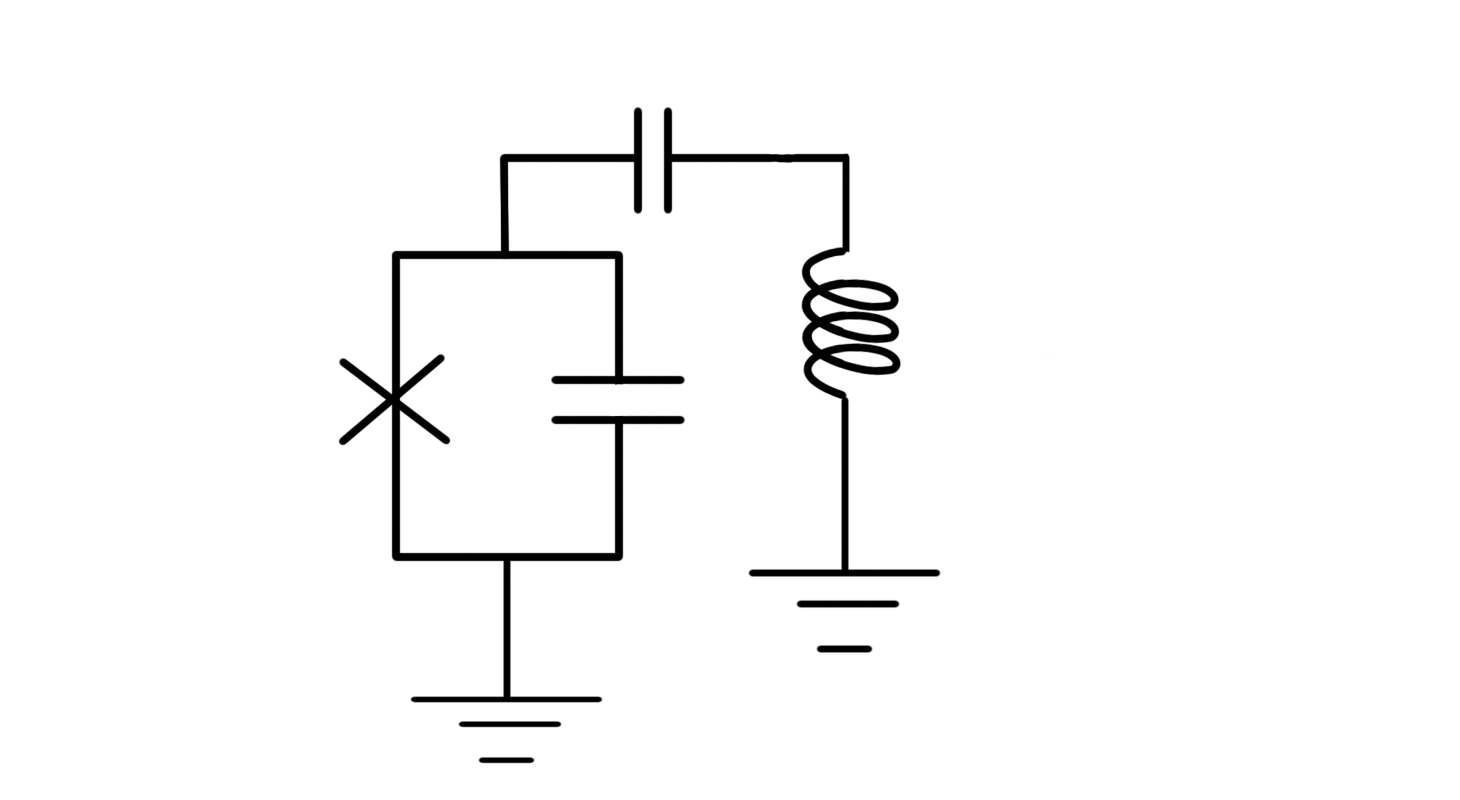
\includegraphics[width=7cm]{TexFigure/kps_singlebath.png}}
  \caption{Brief circuit scheme for single bath condition. The crossing symbol  refers to the insulated junction of Josephson junction.}
\end{figure}
\begin{figure}[htbp]
  \centerline{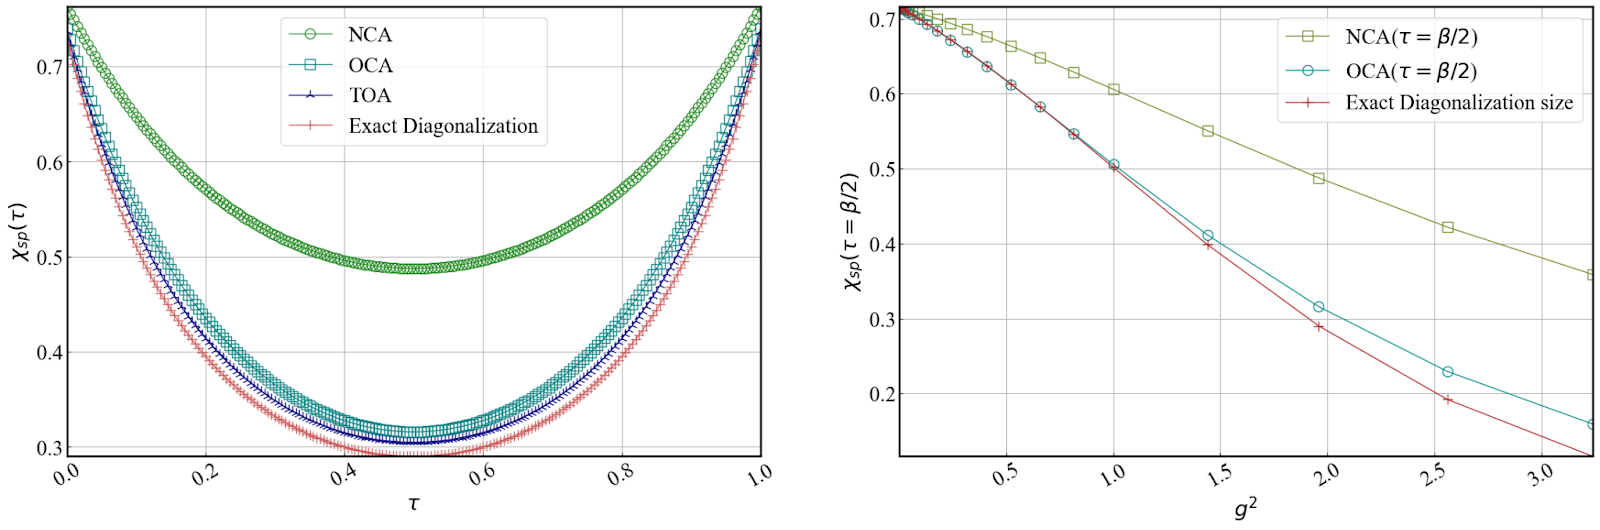
\includegraphics[width=15cm]{TexFigure/bench_single_two.png}}
  \caption{Result for single bath benchmark. For $\chi_{sp} - \tau$(Left), it conducted on overall condition g (coupling strength with system-bath) = 1.
  With $\chi_{sp}(\tau=\beta/2)-g^2$(Right), It shows that if order of perturbation increases, the results approach the exact results.}
\end{figure}
\subsubsection*{Multi-mode case}
To investigate the convergence of the diagrammatic approximation method in a general bosonic reservoir condition, 
we calculated the order parameter and the correlation function using the NCA, OCA, and TOA. 
The results showed no significant difference between the OCA and TOA calculations, confirming that the OCA is a sufficiently convergent method.
\begin{figure}[H]
  \centerline{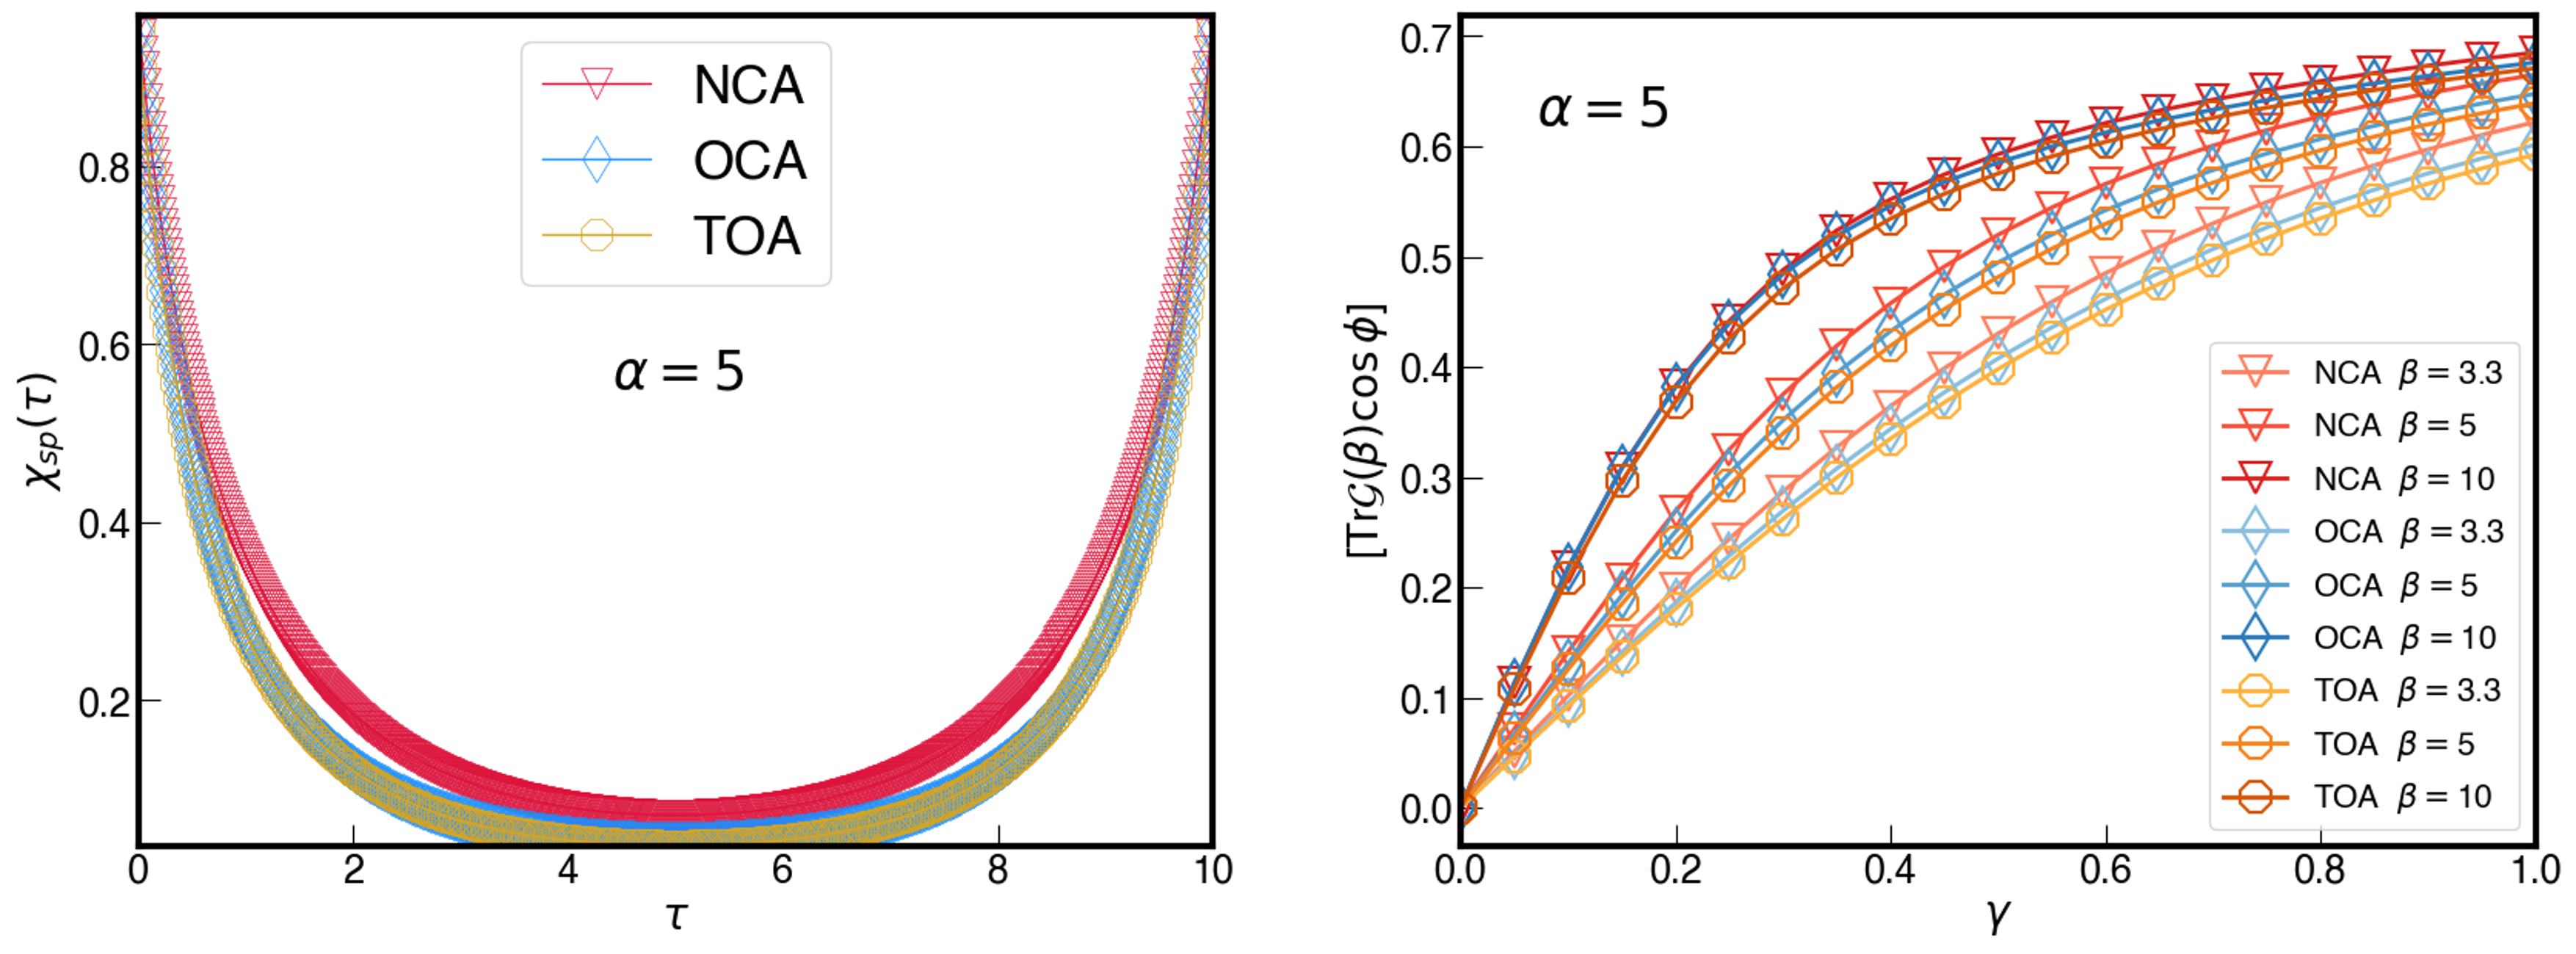
\includegraphics[width=15cm]{TexFigure/Multi_bench.png}}
  \caption{ Calculation results of the order parameter and correlation function using each order of the approximation method. 
  Both figures are for the case of $\alpha$=5, with the left figure showing temperatures between 0.3 and 0.1, 
  the right figure is for the temperature condition of 0.1. It can be observed that the calculation results of OCA and TOA are converged. 
  The size of the τ grid used for the calculation is 701.}
\end{figure}
\subsubsection*{Benchmarking solver code in $\alpha$ = 0 condition}
To check for the integration code, we compared the order parameter calculated using approximation methods for the case of α=0 
with the order parameter calculated using the state density matrix of the Josephson junction system. 
The results showed that the two cases were completely consistent.
\begin{figure}[H]
  \centerline{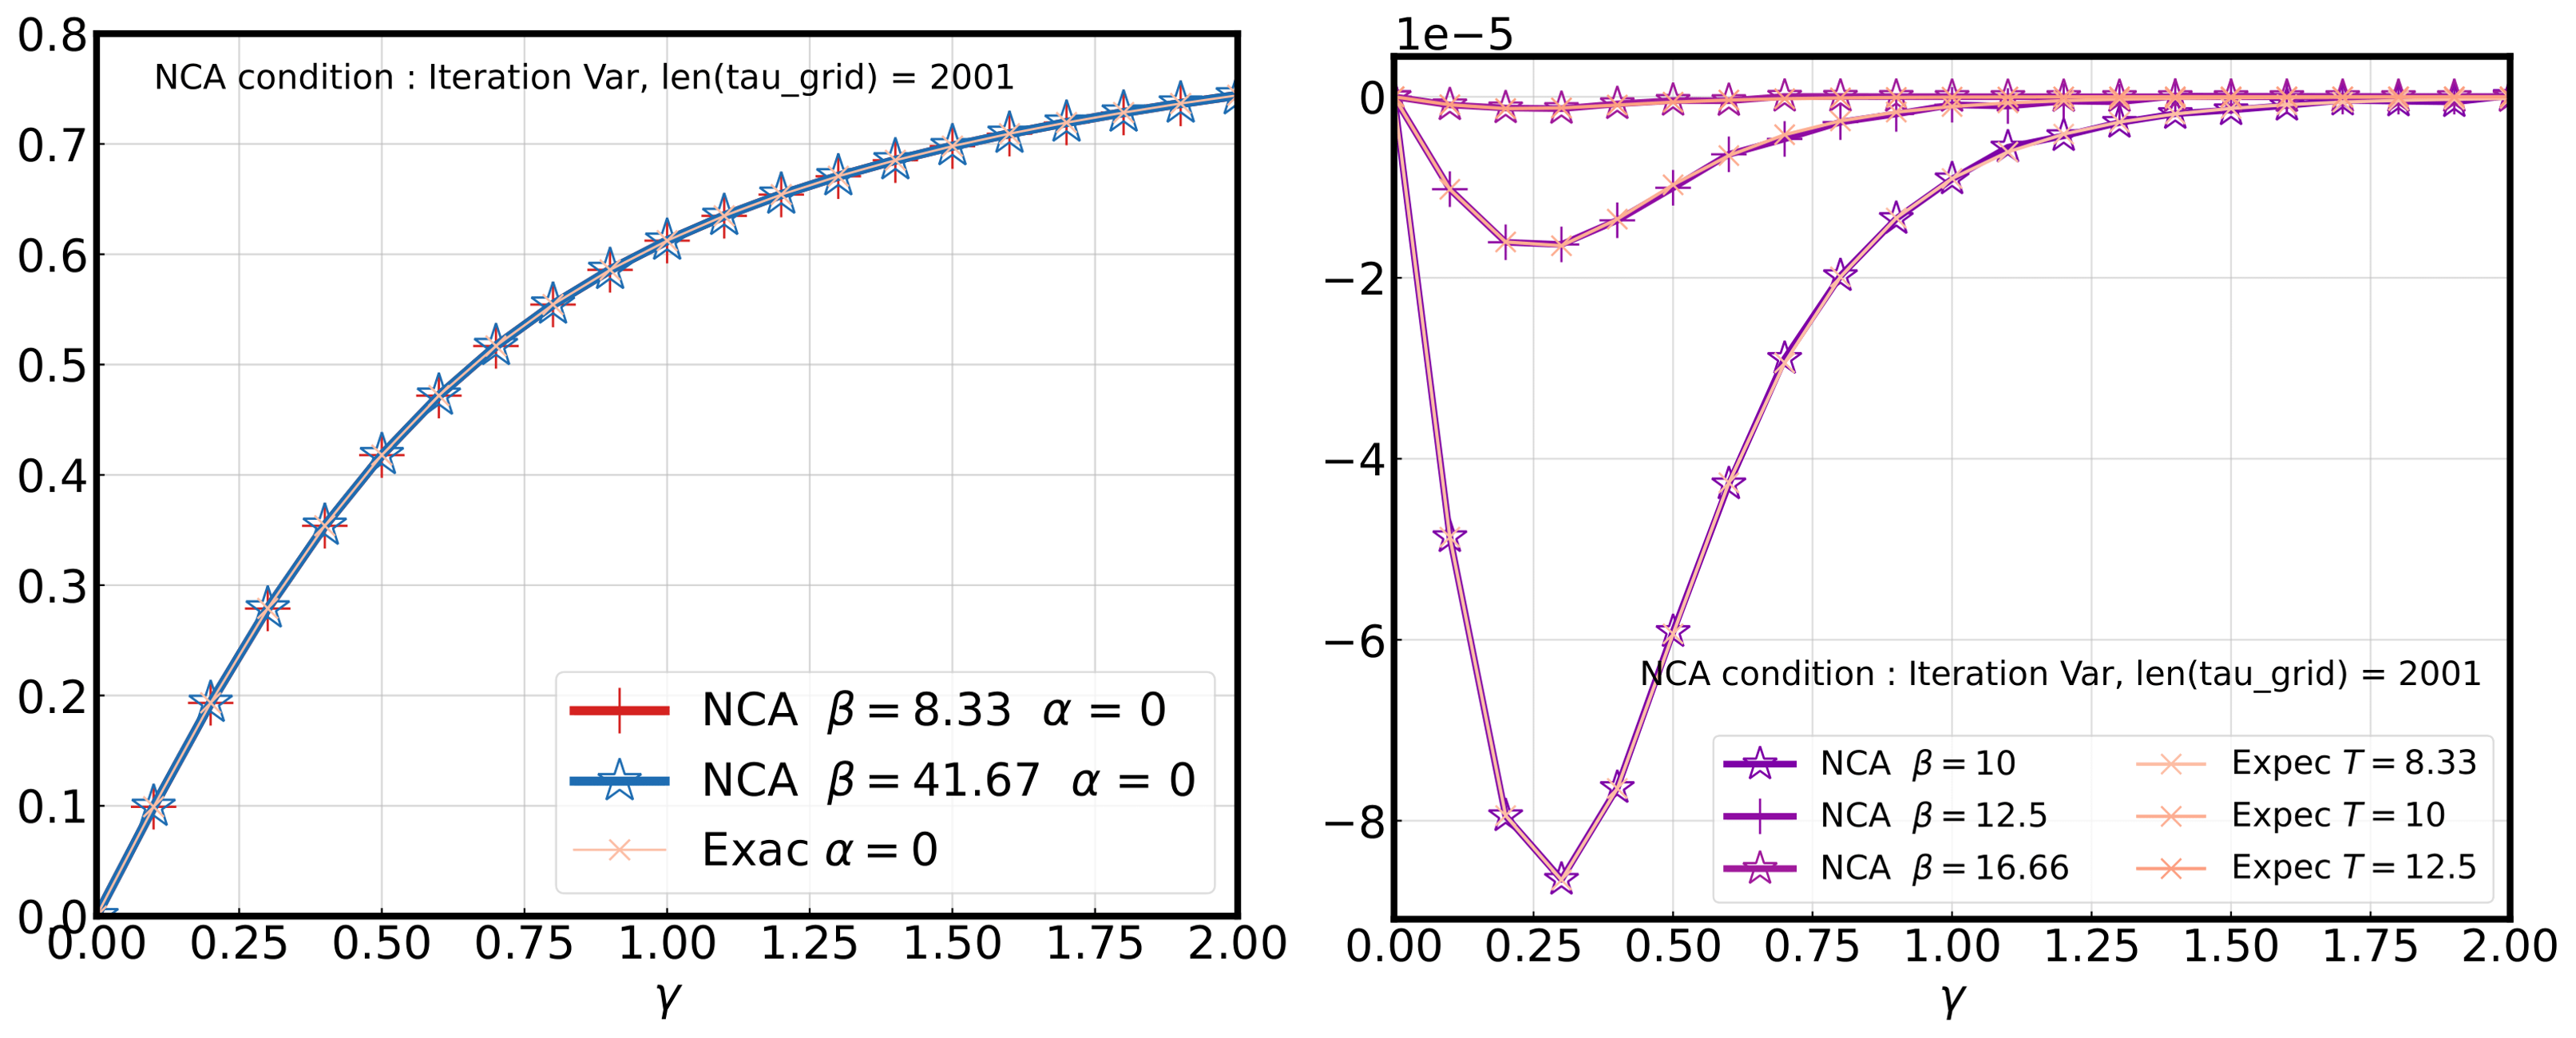
\includegraphics[width=15cm]{TexFigure/Dens_comp.png}}
  \caption{In the case of $\alpha = 0$, order parameter calculation using the approximation method should be consistent with using $H_{loc}$.
  The comparison confirmed that the two cases show consistency. The left figure shows the calculation of the order parameter, 
  and the right figure shows the difference in the order parameter for consecutive $\beta$ values,
   in the intervals [8.33, 10], [10, 12.5], and [12.5, 16.6].}
\end{figure}
\pagebreak
\subsection{Simulation condition}
The control parameters are as follows: $\gamma$ represents the nonlinearity of the Josephson junction system, 
$\alpha$ represents the interaction with the external environment.Regarding the previous study which has been reported 
that the transition occurs at $\alpha = 1$, we set the range of parameters around $\alpha = 1$ and $\gamma = 1$ . 
The factors influencing the accuracy of the approximation method are the number of integration iterations and the size of the $\tau$ grid. 
We set the range of variables used in the simulation as Table 2 and Table 3.
\begin{table}[htbp]
  \centering
  \renewcommand{\arraystretch}{1.2}  % 행 간격 조정
  \begin{tabular}{@{}cccc@{}}
  \toprule
  \textbf{Variables} & \textbf{Min} & \textbf{Max}  & \textbf{Interval}\\ 
  \midrule
  $\gamma$ & 0 & 2 & 0.1 \\
  $\alpha$ & 0 & 2 & 0.01 \\
  $\beta$ & 7.14 & 62.5 &  \\
  Temperature & 0.016 & 0.14 & 0.02 (until 0.04) \\
  \bottomrule
  \end{tabular}
  \caption{Parameter interval used for calculation.}
  \end{table}
\begin{table}[htbp]
  \centering
  \renewcommand{\arraystretch}{1.2}  % 행 간격 조정
  \begin{tabular}{@{}ccc@{}}
  \toprule
  \textbf{Number} & \textbf{Interval} & \textbf{Gridsize}\\ 
  \midrule
  $\tau$ grid & [0,$\beta$] & 2000 \\
  k grid & [0,K = 30000] & 30000 \\
  \bottomrule
  \end{tabular}
  \caption{Grid condition used for calculation.}
  \end{table}
\subsubsection*{Saturation test}
We investigated the convergence behavior of the calculation results for the change of the order parameter. 
We were able to confirm that the results converge for the case of a tau grid size of 1800 to 2000. 
\begin{figure}[htbp]
  \centerline{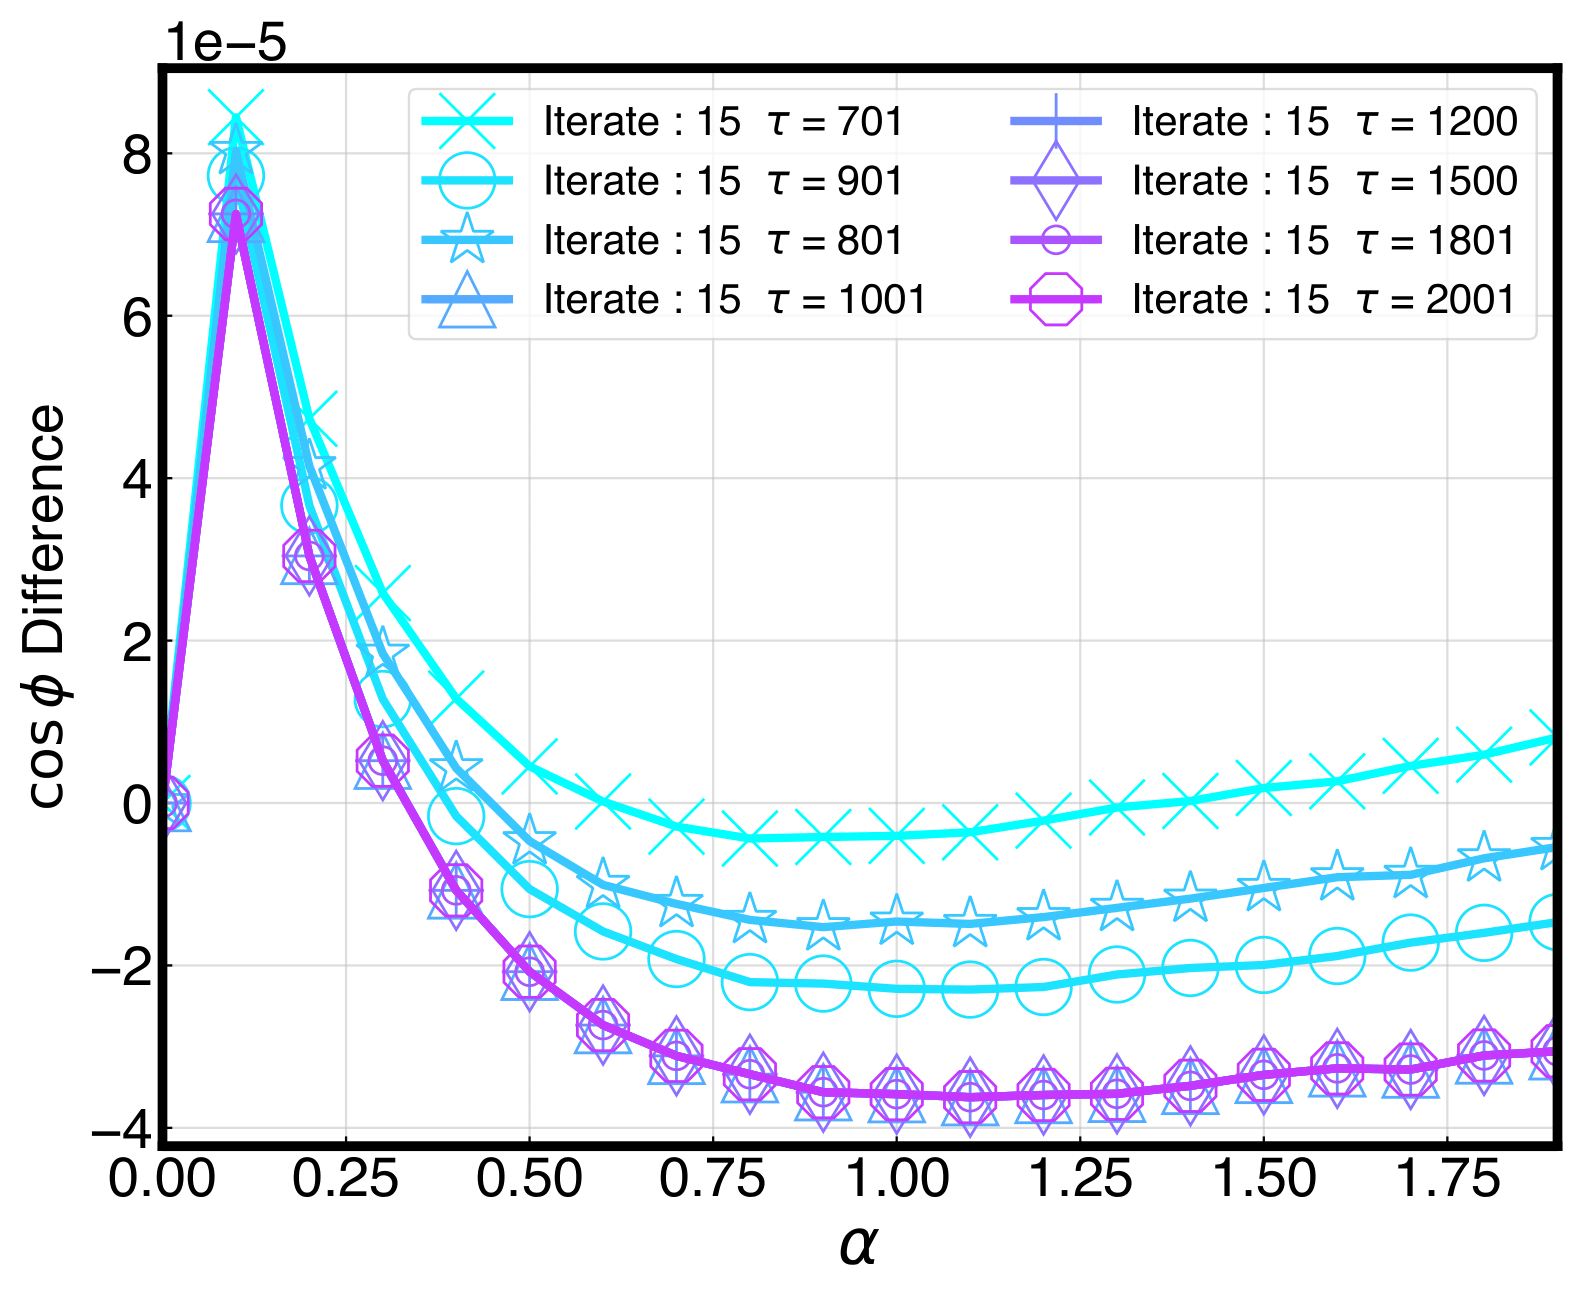
\includegraphics[width=10cm]{TexFigure/Diff_Ns3_g_b_35.71_41.67_n_15_tauchange (1)-1.png}}
  \caption{Saturation test in different time grid size. The temperature condition is $\beta = 41.67$}
\end{figure}
\subsubsection*{Size dependence}
Since the resistively shunted Josephson junction circuit corresponds to a model that the physical system has coupled to waveguide structure,
there was a breakdown of the rotating wave approximation of the two-level system as the coupling strength between the RC resonator circuit 
and the Josephson junction increases.The test condition is $\gamma =2$ , $\alpha = 1.5$ with calculating correlation function. 
From the benchmark result, adopting 2-level truncated condition is reliable since the difference between two size is ignorable.
\begin{figure}[H]
  \centerline{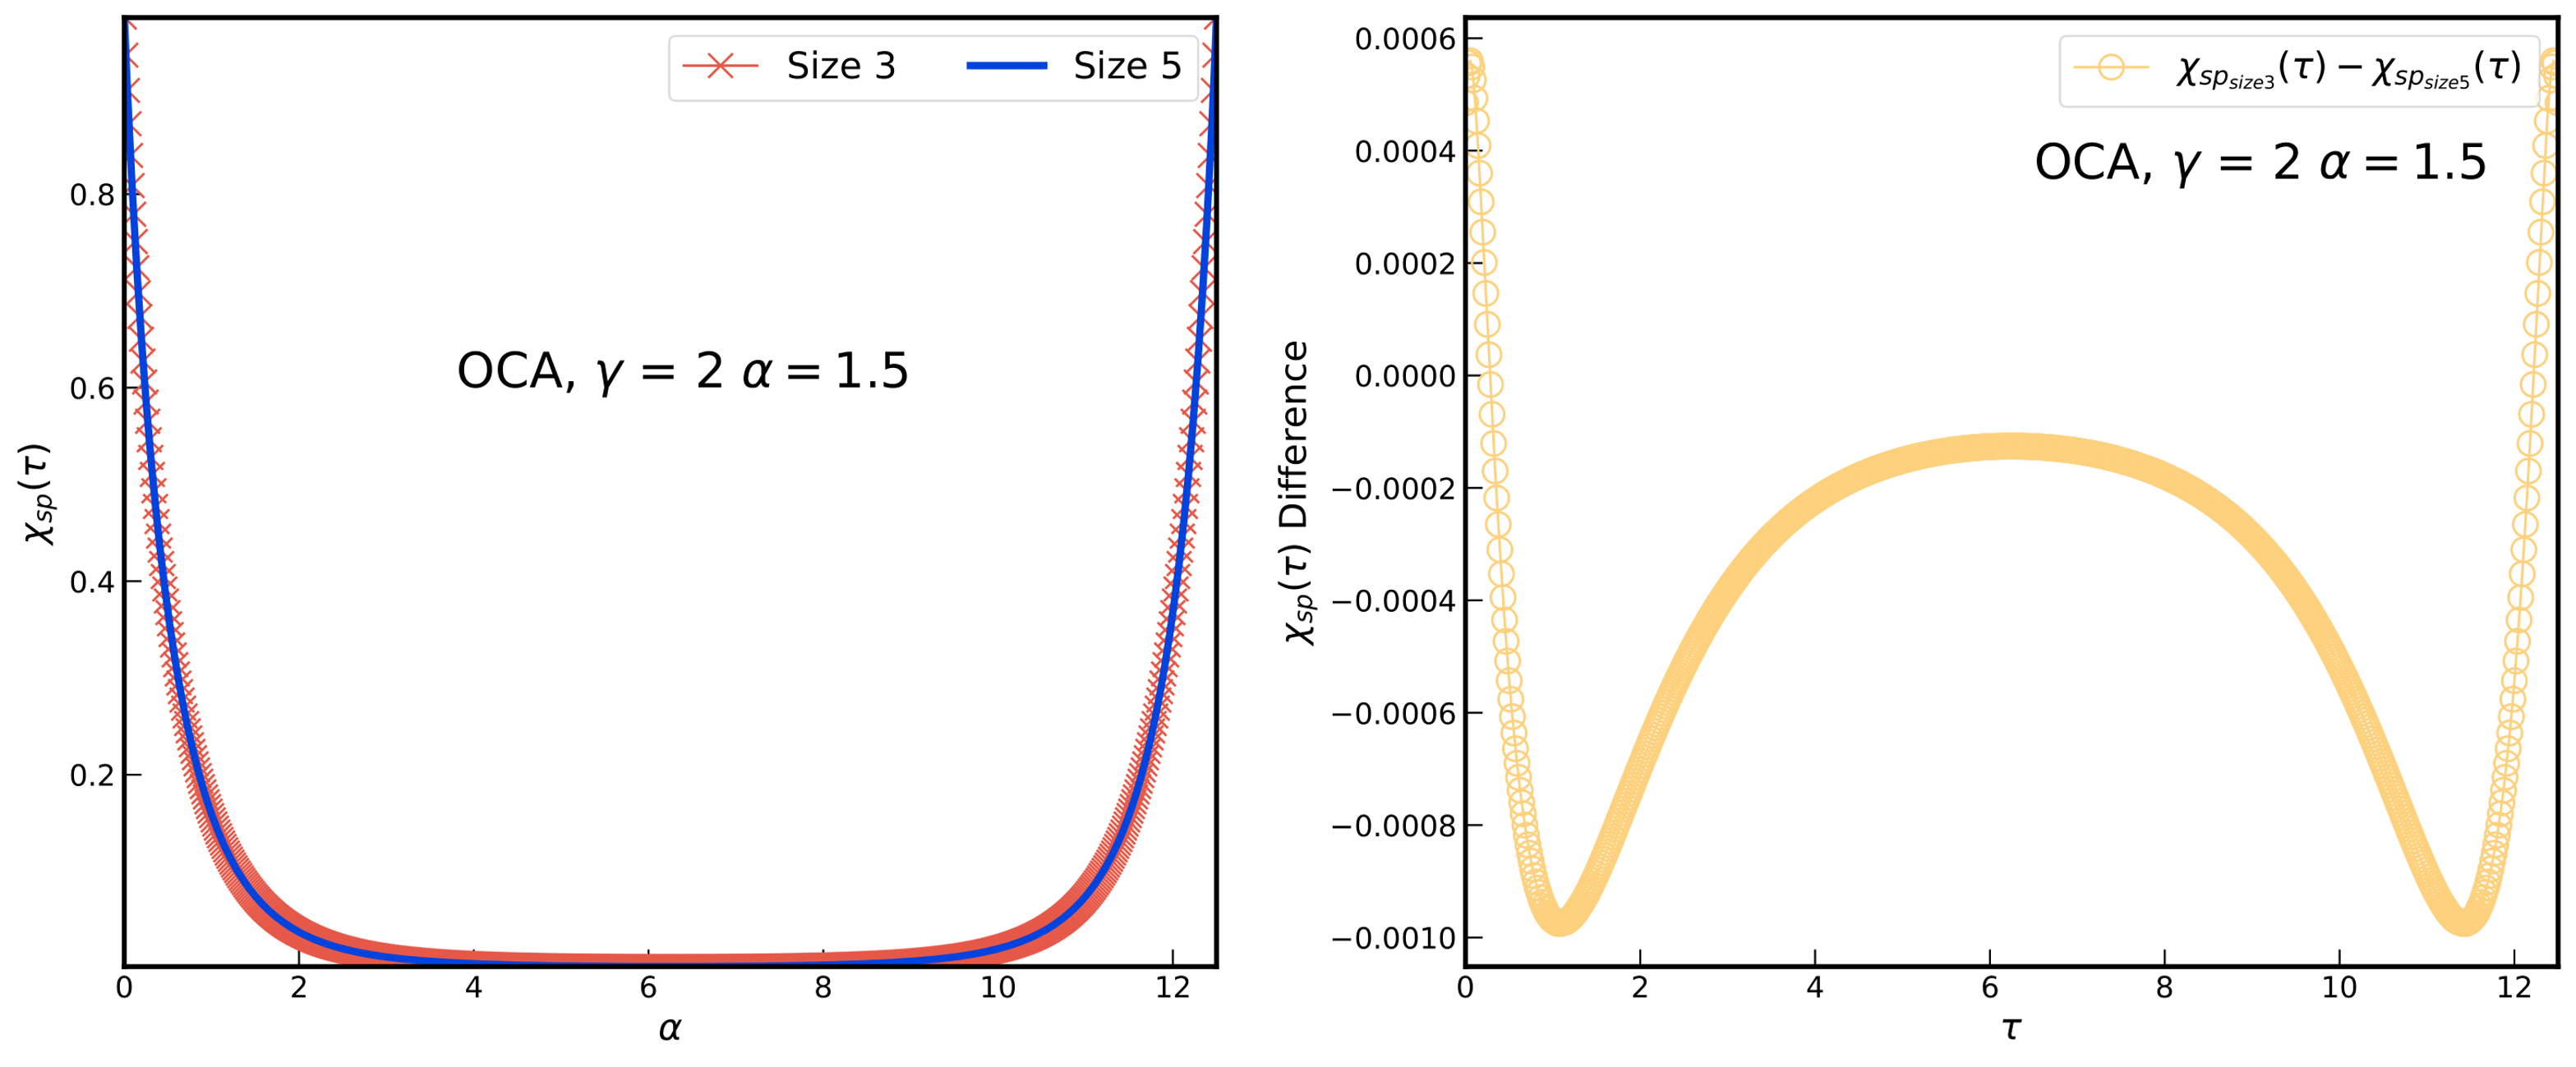
\includegraphics[width=15cm]{TexFigure/Sizediff.png}}
  \caption{Comparision with $\chi_{sp}(\tau)$ size3 and size5. The size of $\tau$ grid is 700.}
\end{figure}
\pagebreak
\subsection{Orderparmeter}
We calculated the expectation value of the order parameter, $\cos\phi$ for various temperatures at $\alpha = 0.1$. 
In Figure 16, The results showed that the Josephson junction exhibits superconducting behavior as the nonlinearity increases at all temperatures. 
Subsequently, we examined the diagonal elements of $\cos\phi \cdot e^{−βH_{loc}}$ for $\alpha=$ 0, 0.1, and 1. 
In this case, the diagonal elements represent the system being in the ground state, the even-function form of the first excited state, 
and the odd-function form of the first excited state, respectively. 
For all cases, we confirmed that the system will localized as in the ground state. 
This indicates that the system exhibits superconductivity, consistent with the observed expectation value of the order parameter.\\
\begin{figure}[htbp]
  \centerline{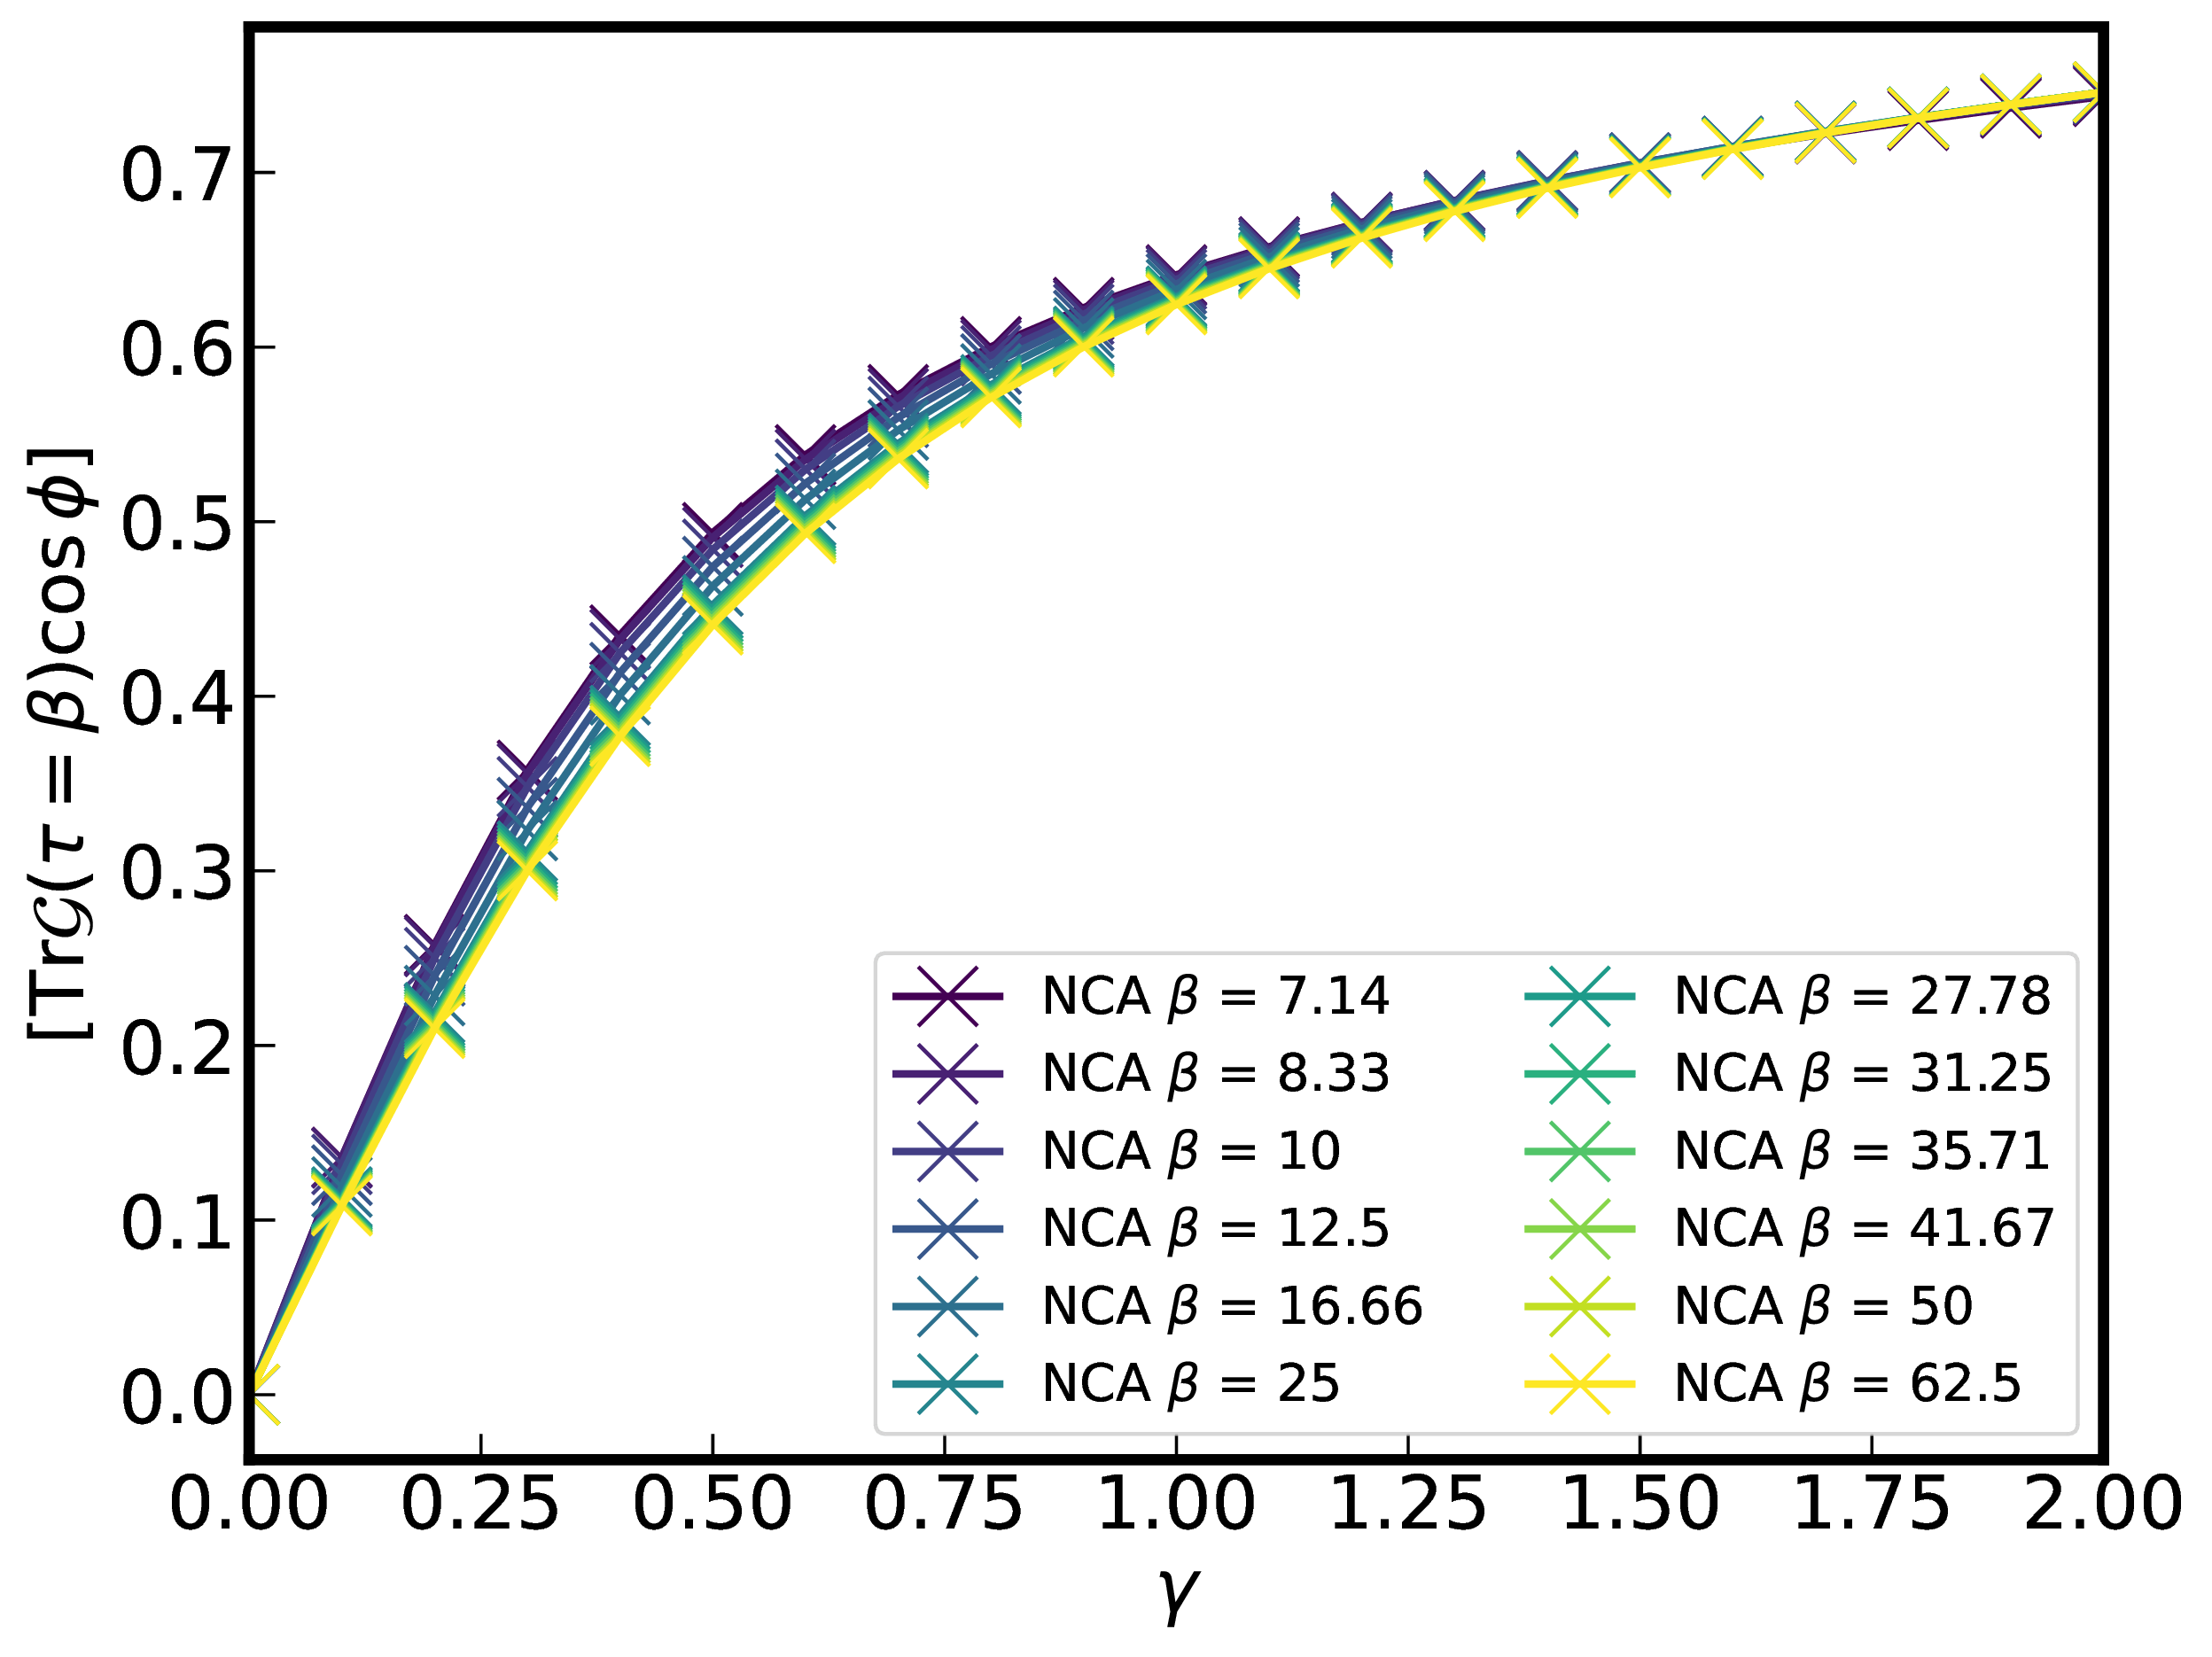
\includegraphics[width=10cm]{TexFigure/Expec_alp_0.1 (1).png}}
  \caption{Result of the expectation of order parameter, $\cos\phi$.}
\end{figure}
\begin{figure}[htbp]
  \centerline{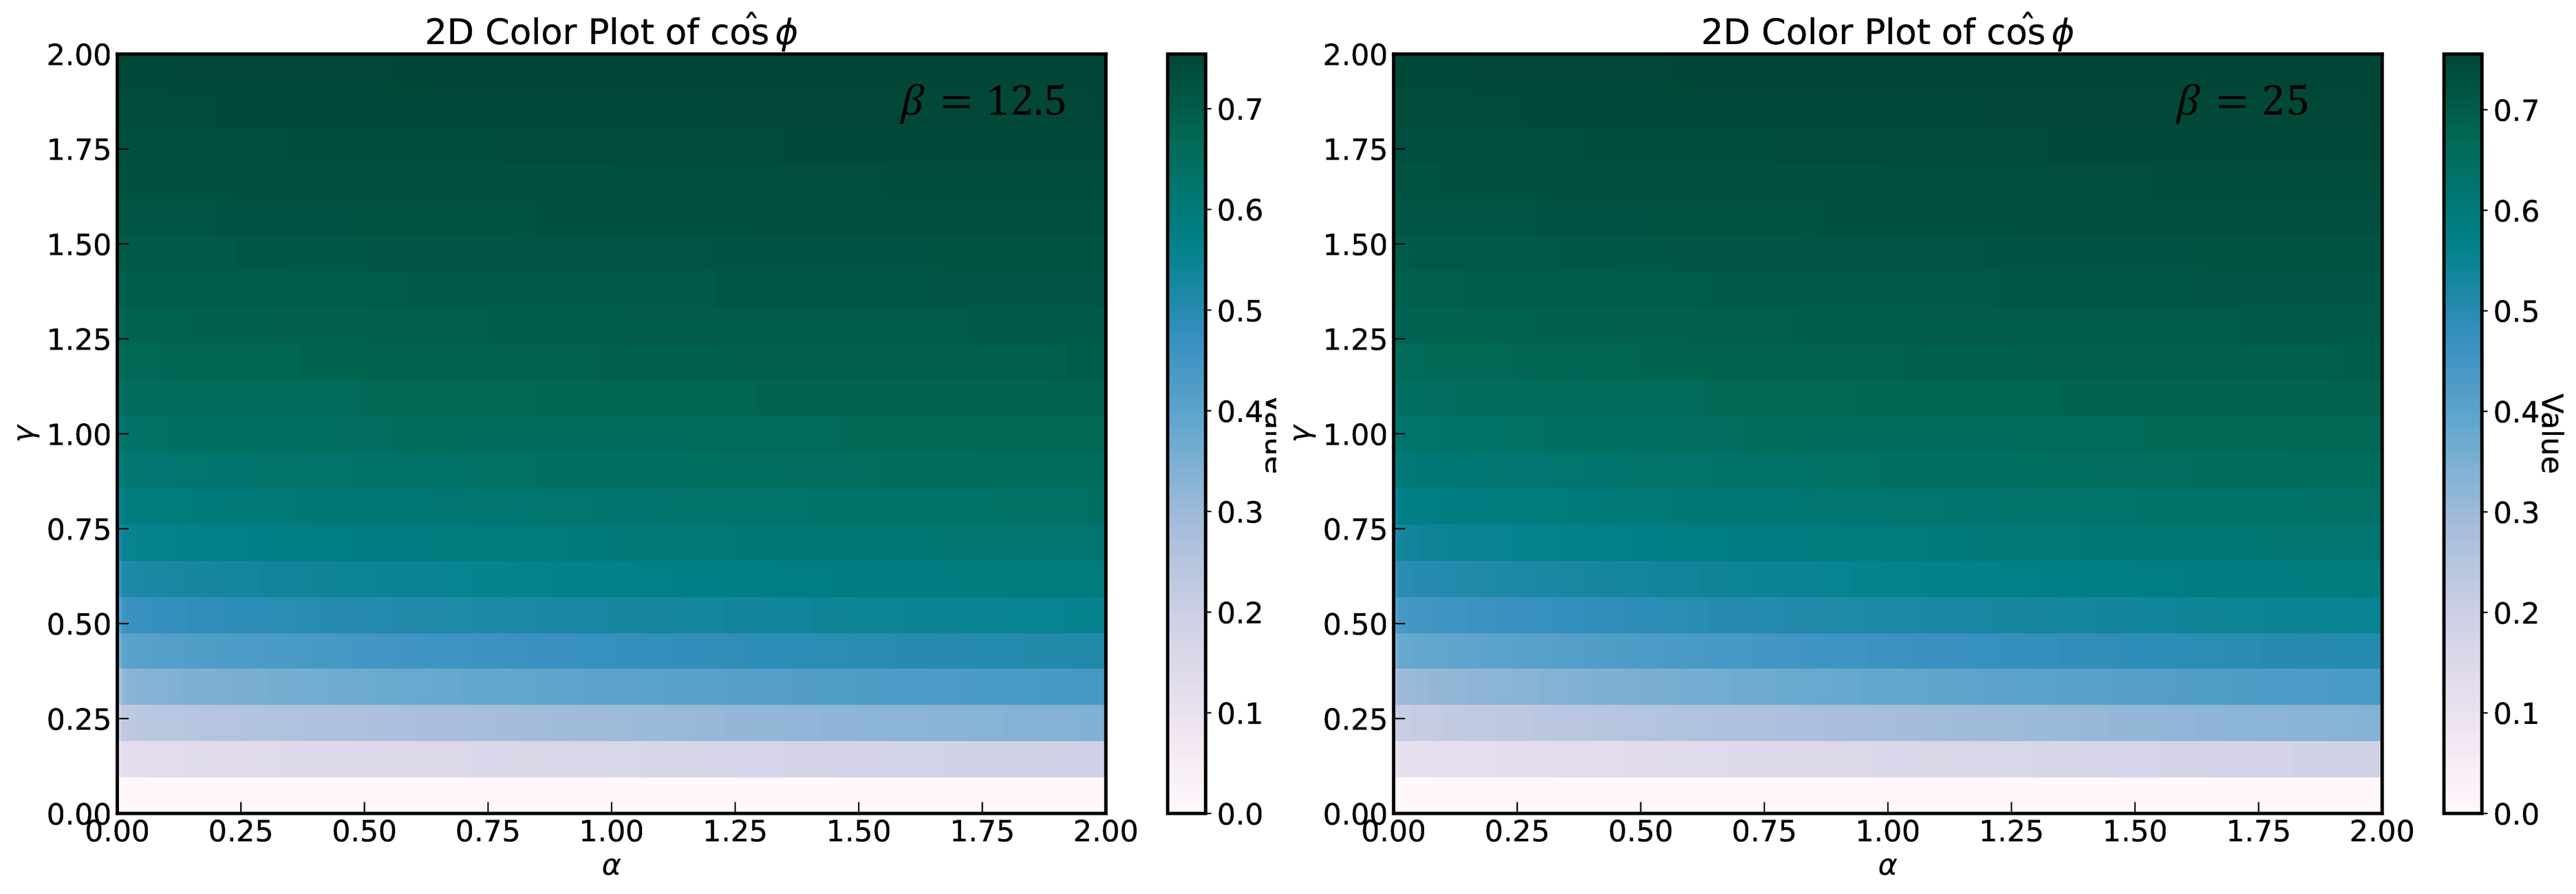
\includegraphics[width=16cm]{TexFigure/Order_color.png}}
  \caption{Colored plot for the expectation value of order parameter. The simulation was performed in NCA. The left figure is in the case of $\beta=10$, Right is for $\beta=25$.
  The difference in phase on each side of the junction goes lower as the color goes deeper.}
\end{figure}
\begin{figure}[H]
  \centerline{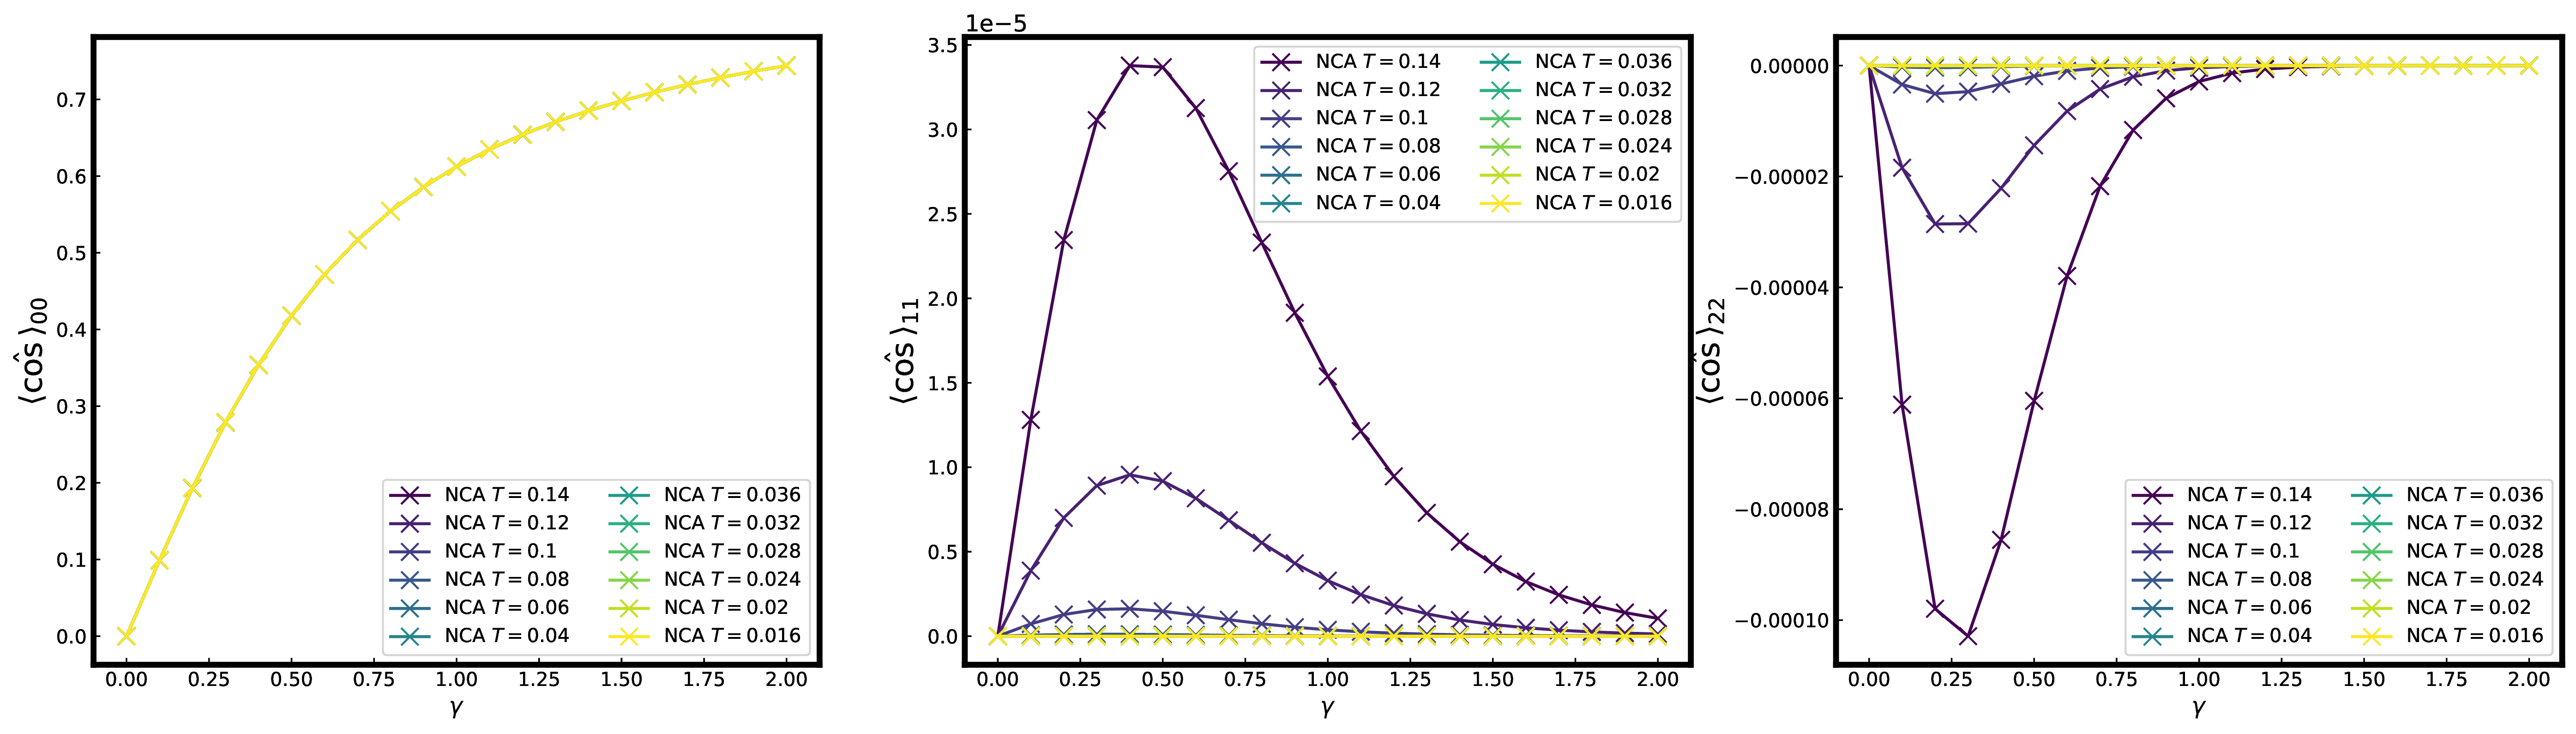
\includegraphics[width=17cm]{TexFigure/Matele_Ns3_alp0.png}}
  \centerline{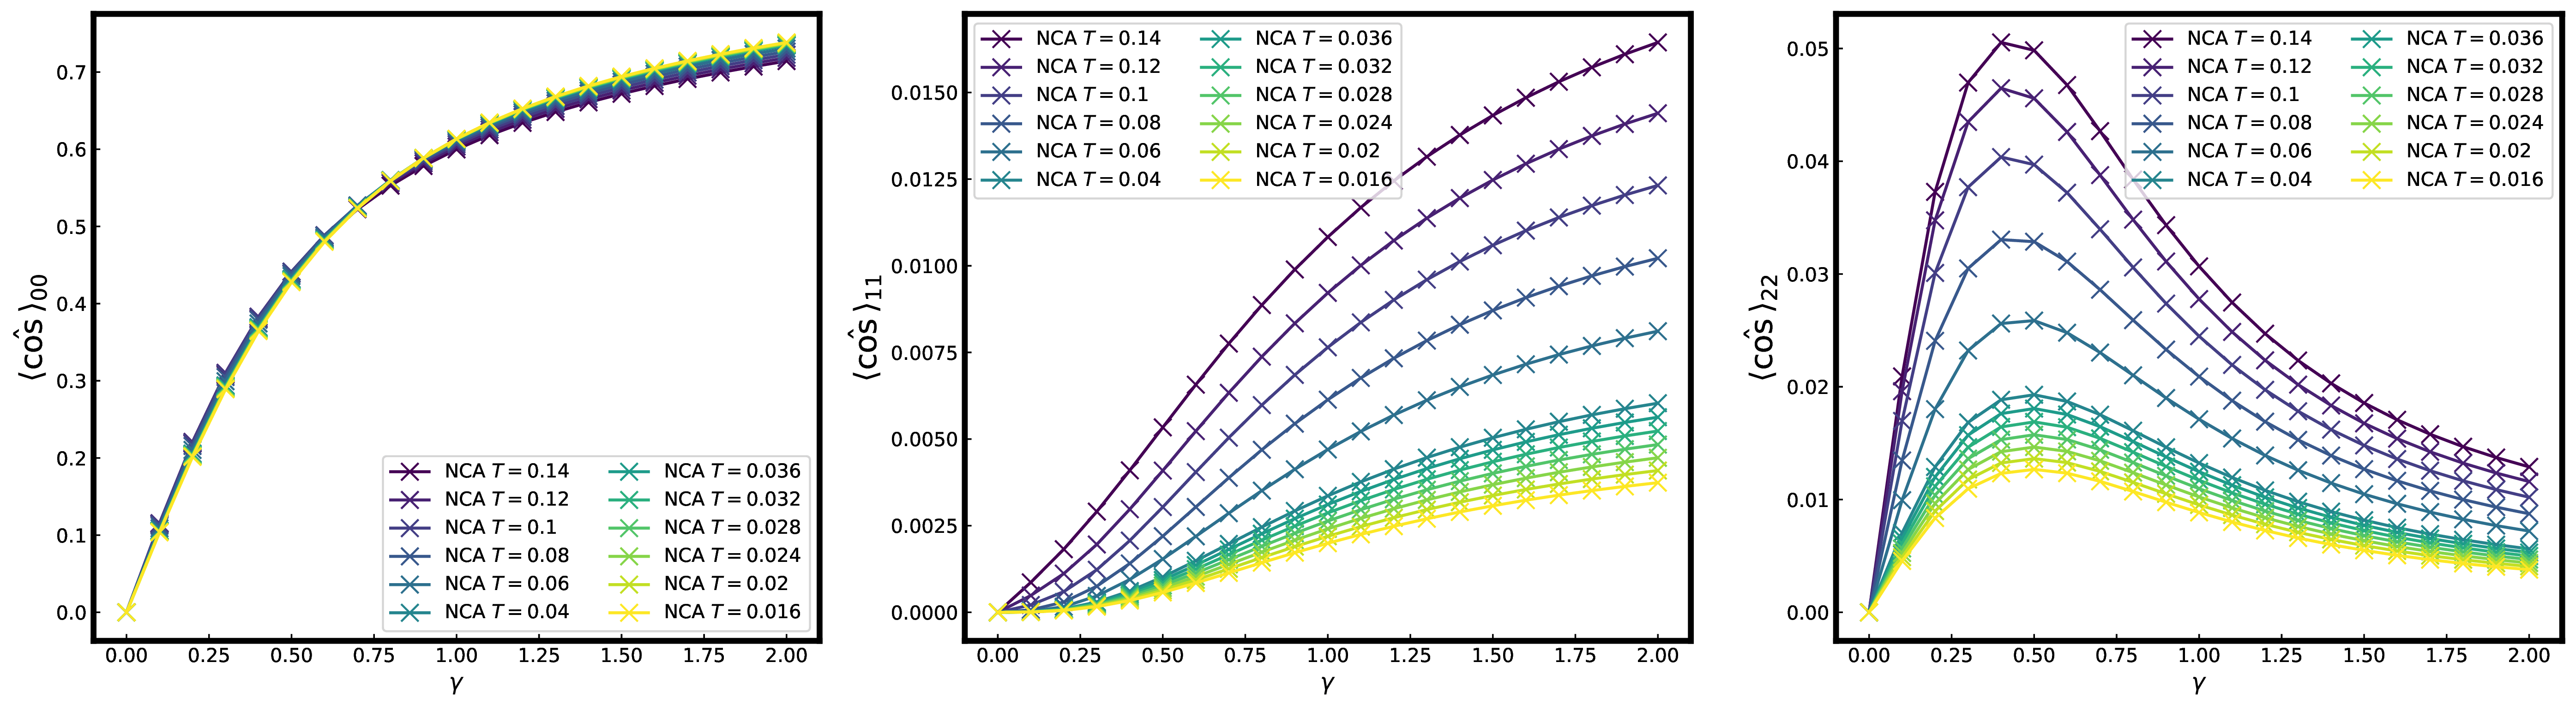
\includegraphics[width=17cm]{TexFigure/Matele_Ns3_alp0_1.png}}
  \centerline{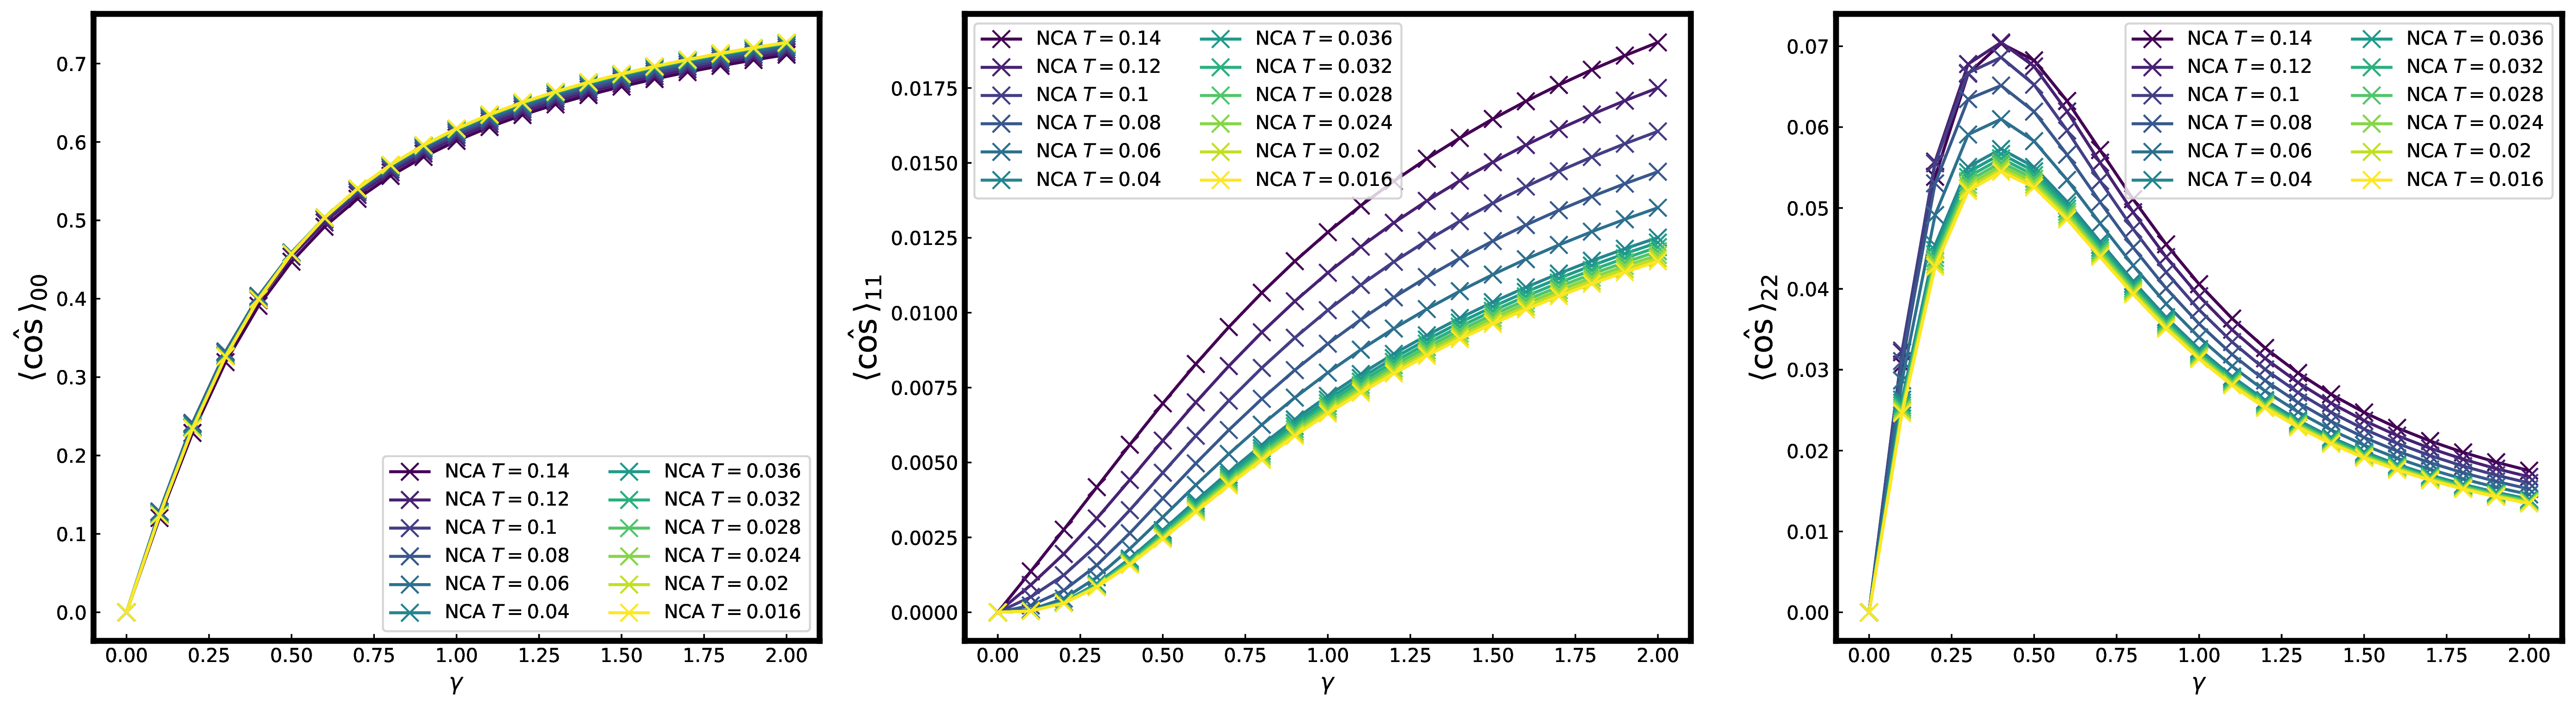
\includegraphics[width=17cm]{TexFigure/Matele_Ns3_alp1.png}}
  \caption{Change of matrix element of matrix multiplication result between $\cos\phi$ and density matrix.}
\end{figure}
\subsubsection*{Temperature dependent criticality}
To confirm the criticality of the system's phase with respect to temperature, 
we observed the change in the order parameter while varying the temperature. As the temperature decreases, 
the rate of change of the order parameter shifts from a high slope to a low slope. 
It can be predicted that a temperature-dependent phase transition occurs at the given point.
\begin{figure}[htbp]
  \centerline{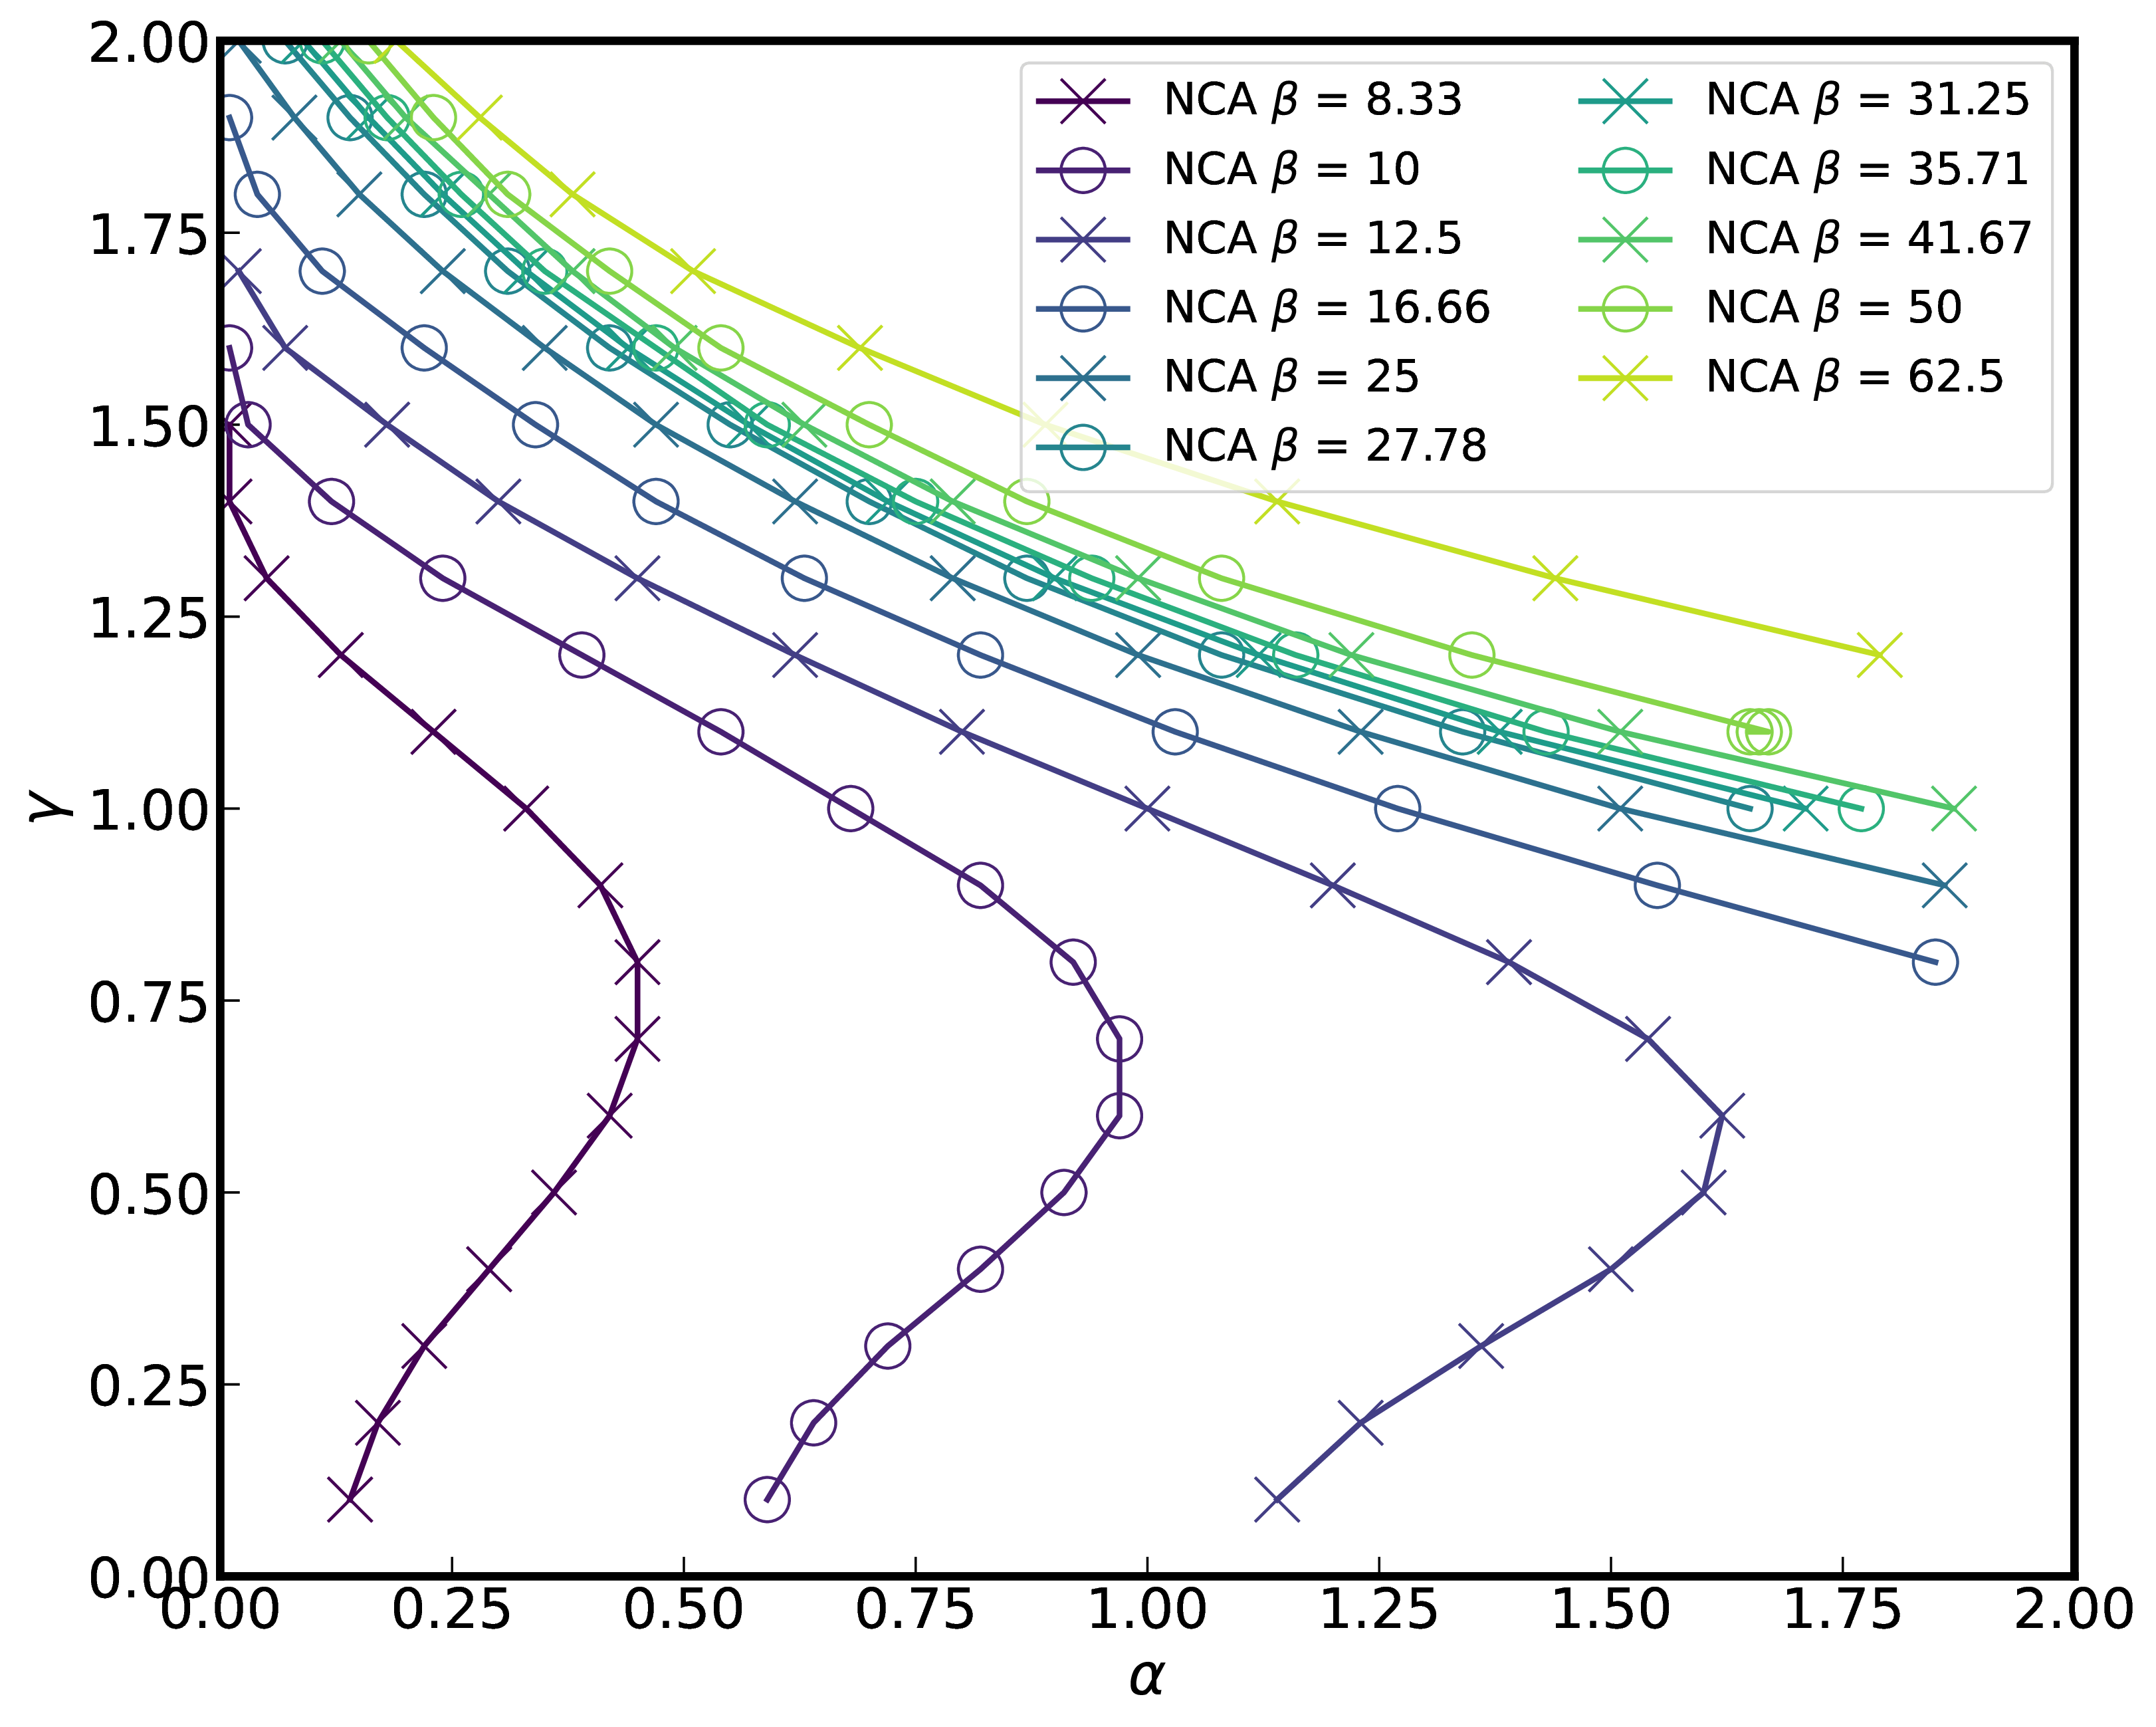
\includegraphics[width=12cm]{TexFigure/3dplot_Ns3_proj_n (2).png}}
  \centerline{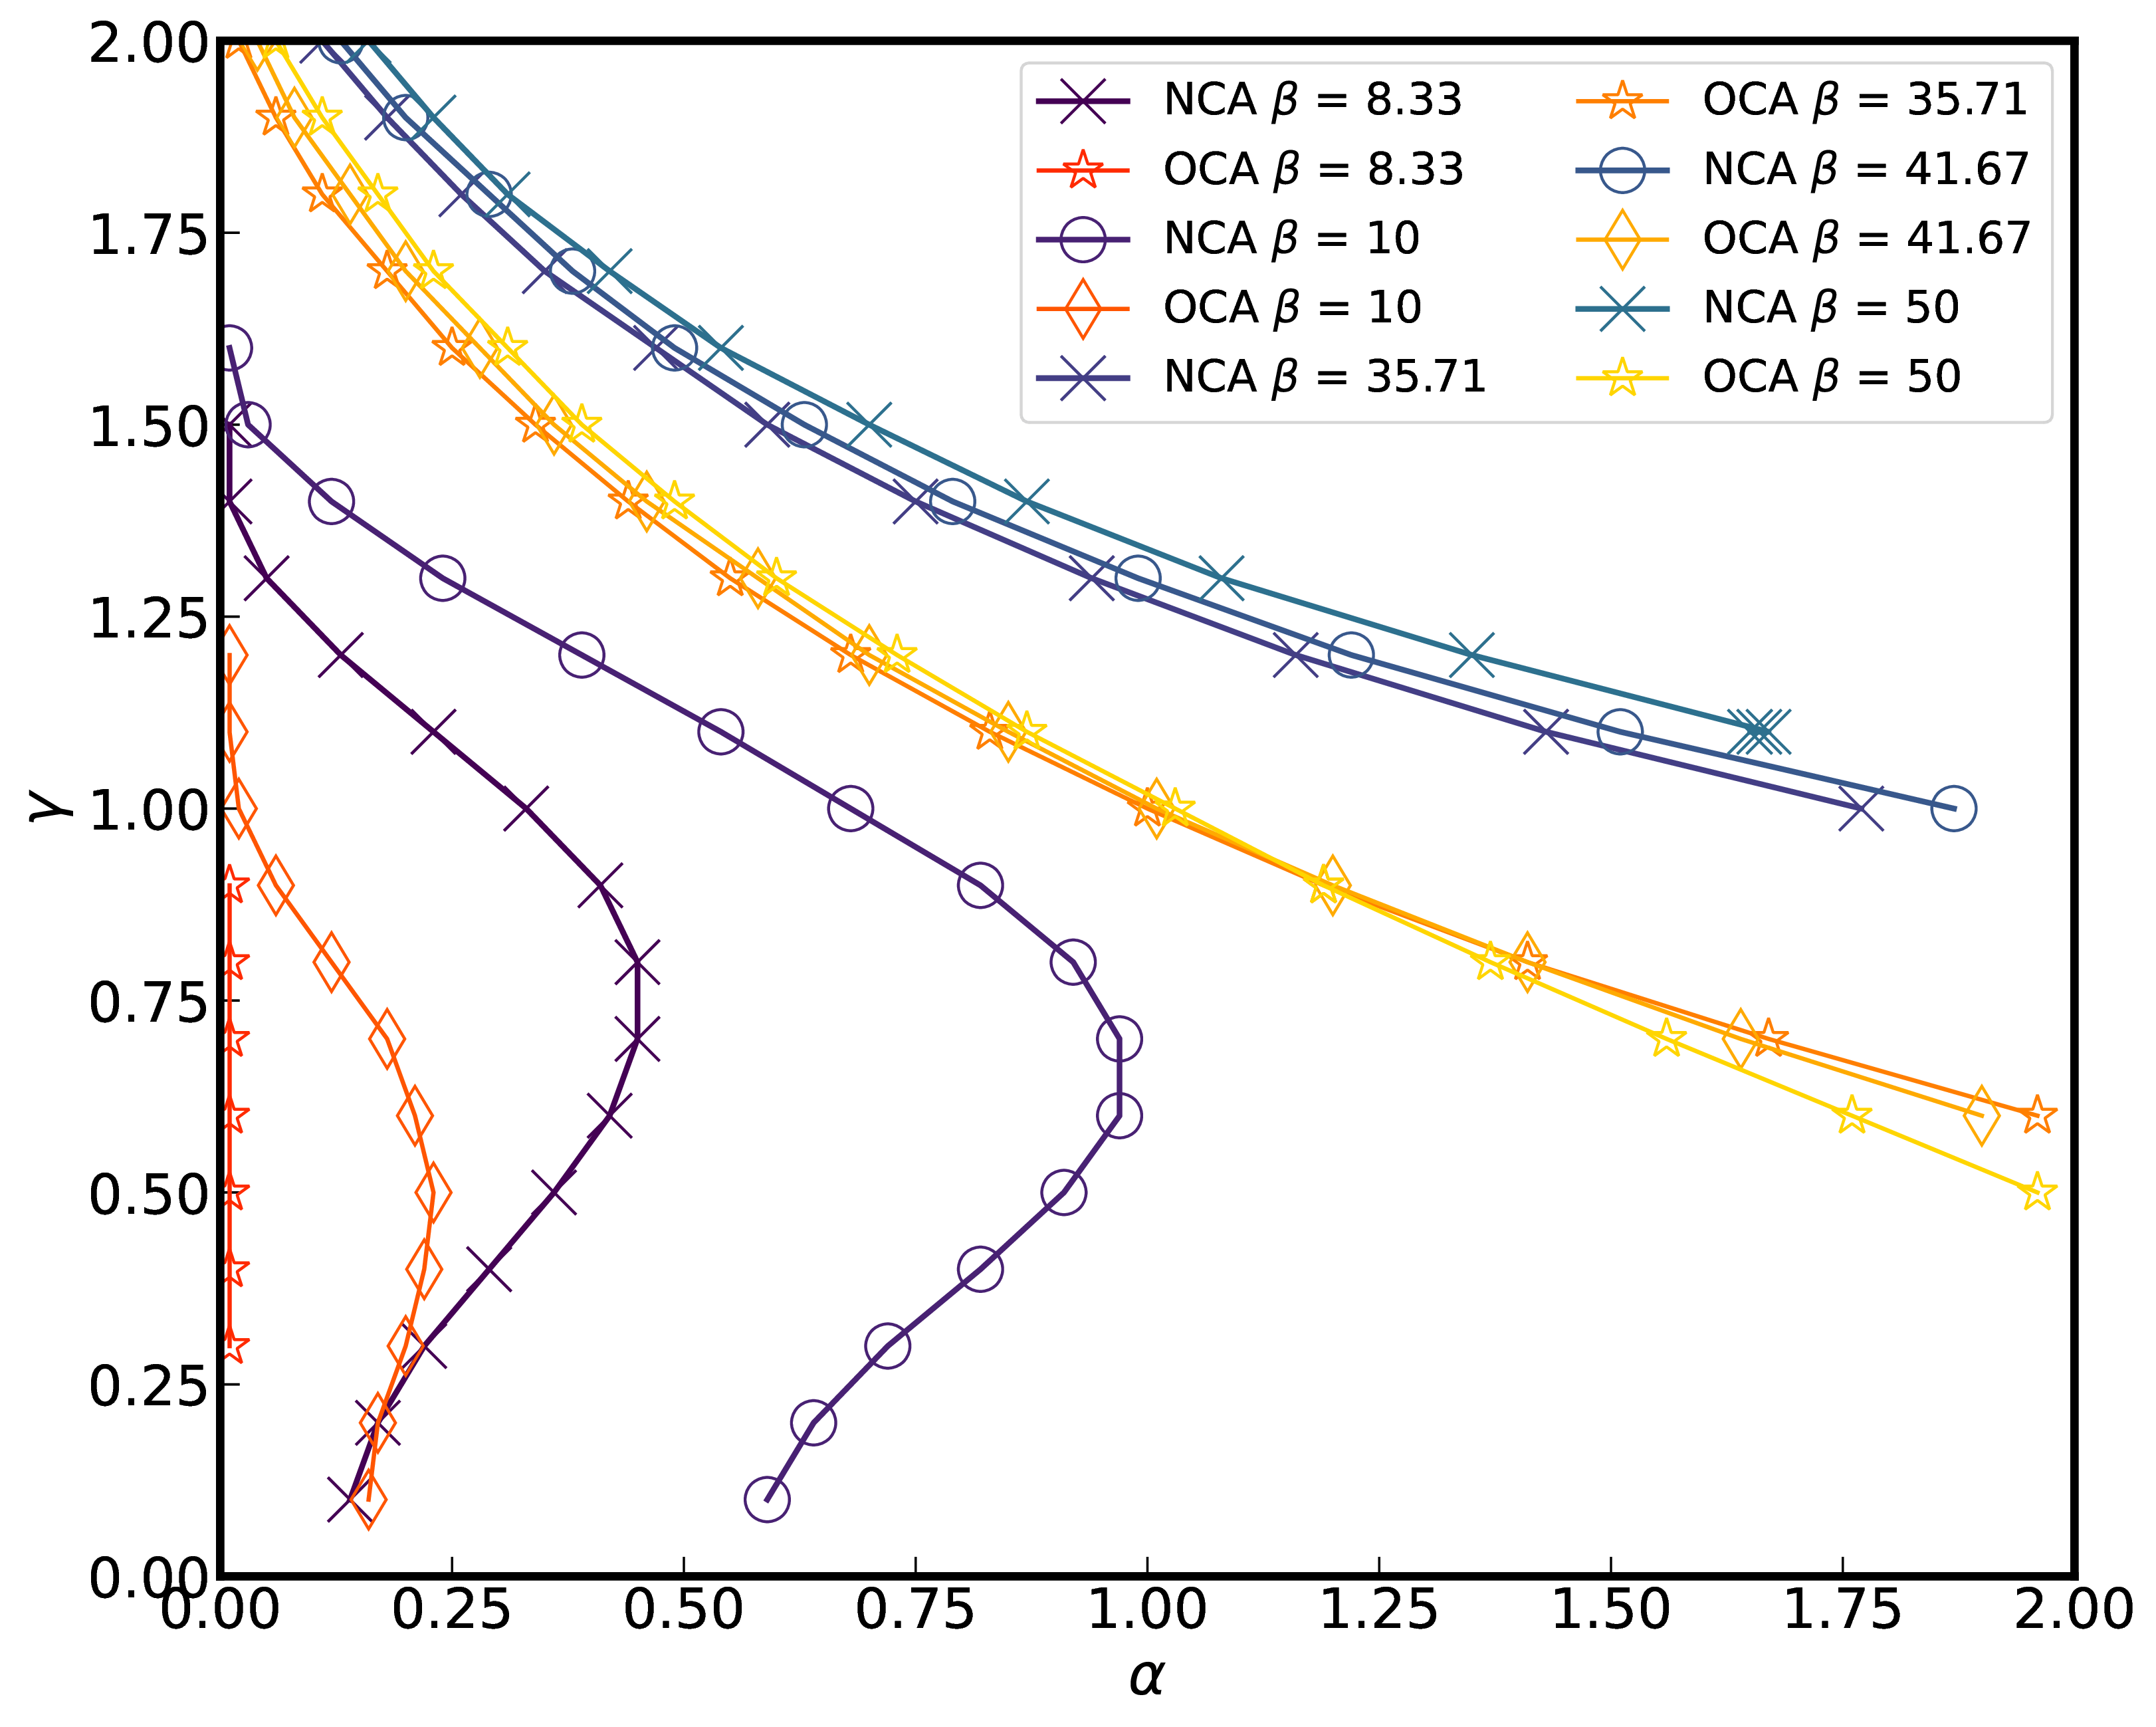
\includegraphics[width=12cm]{TexFigure/3dplot_COMP3_proj_n (2).png}}
  \caption{Figure for finite temperature criticality. Below is the comparision data between NCA and OCA.}
\end{figure}
\begin{figure}[htbp]
  \centerline{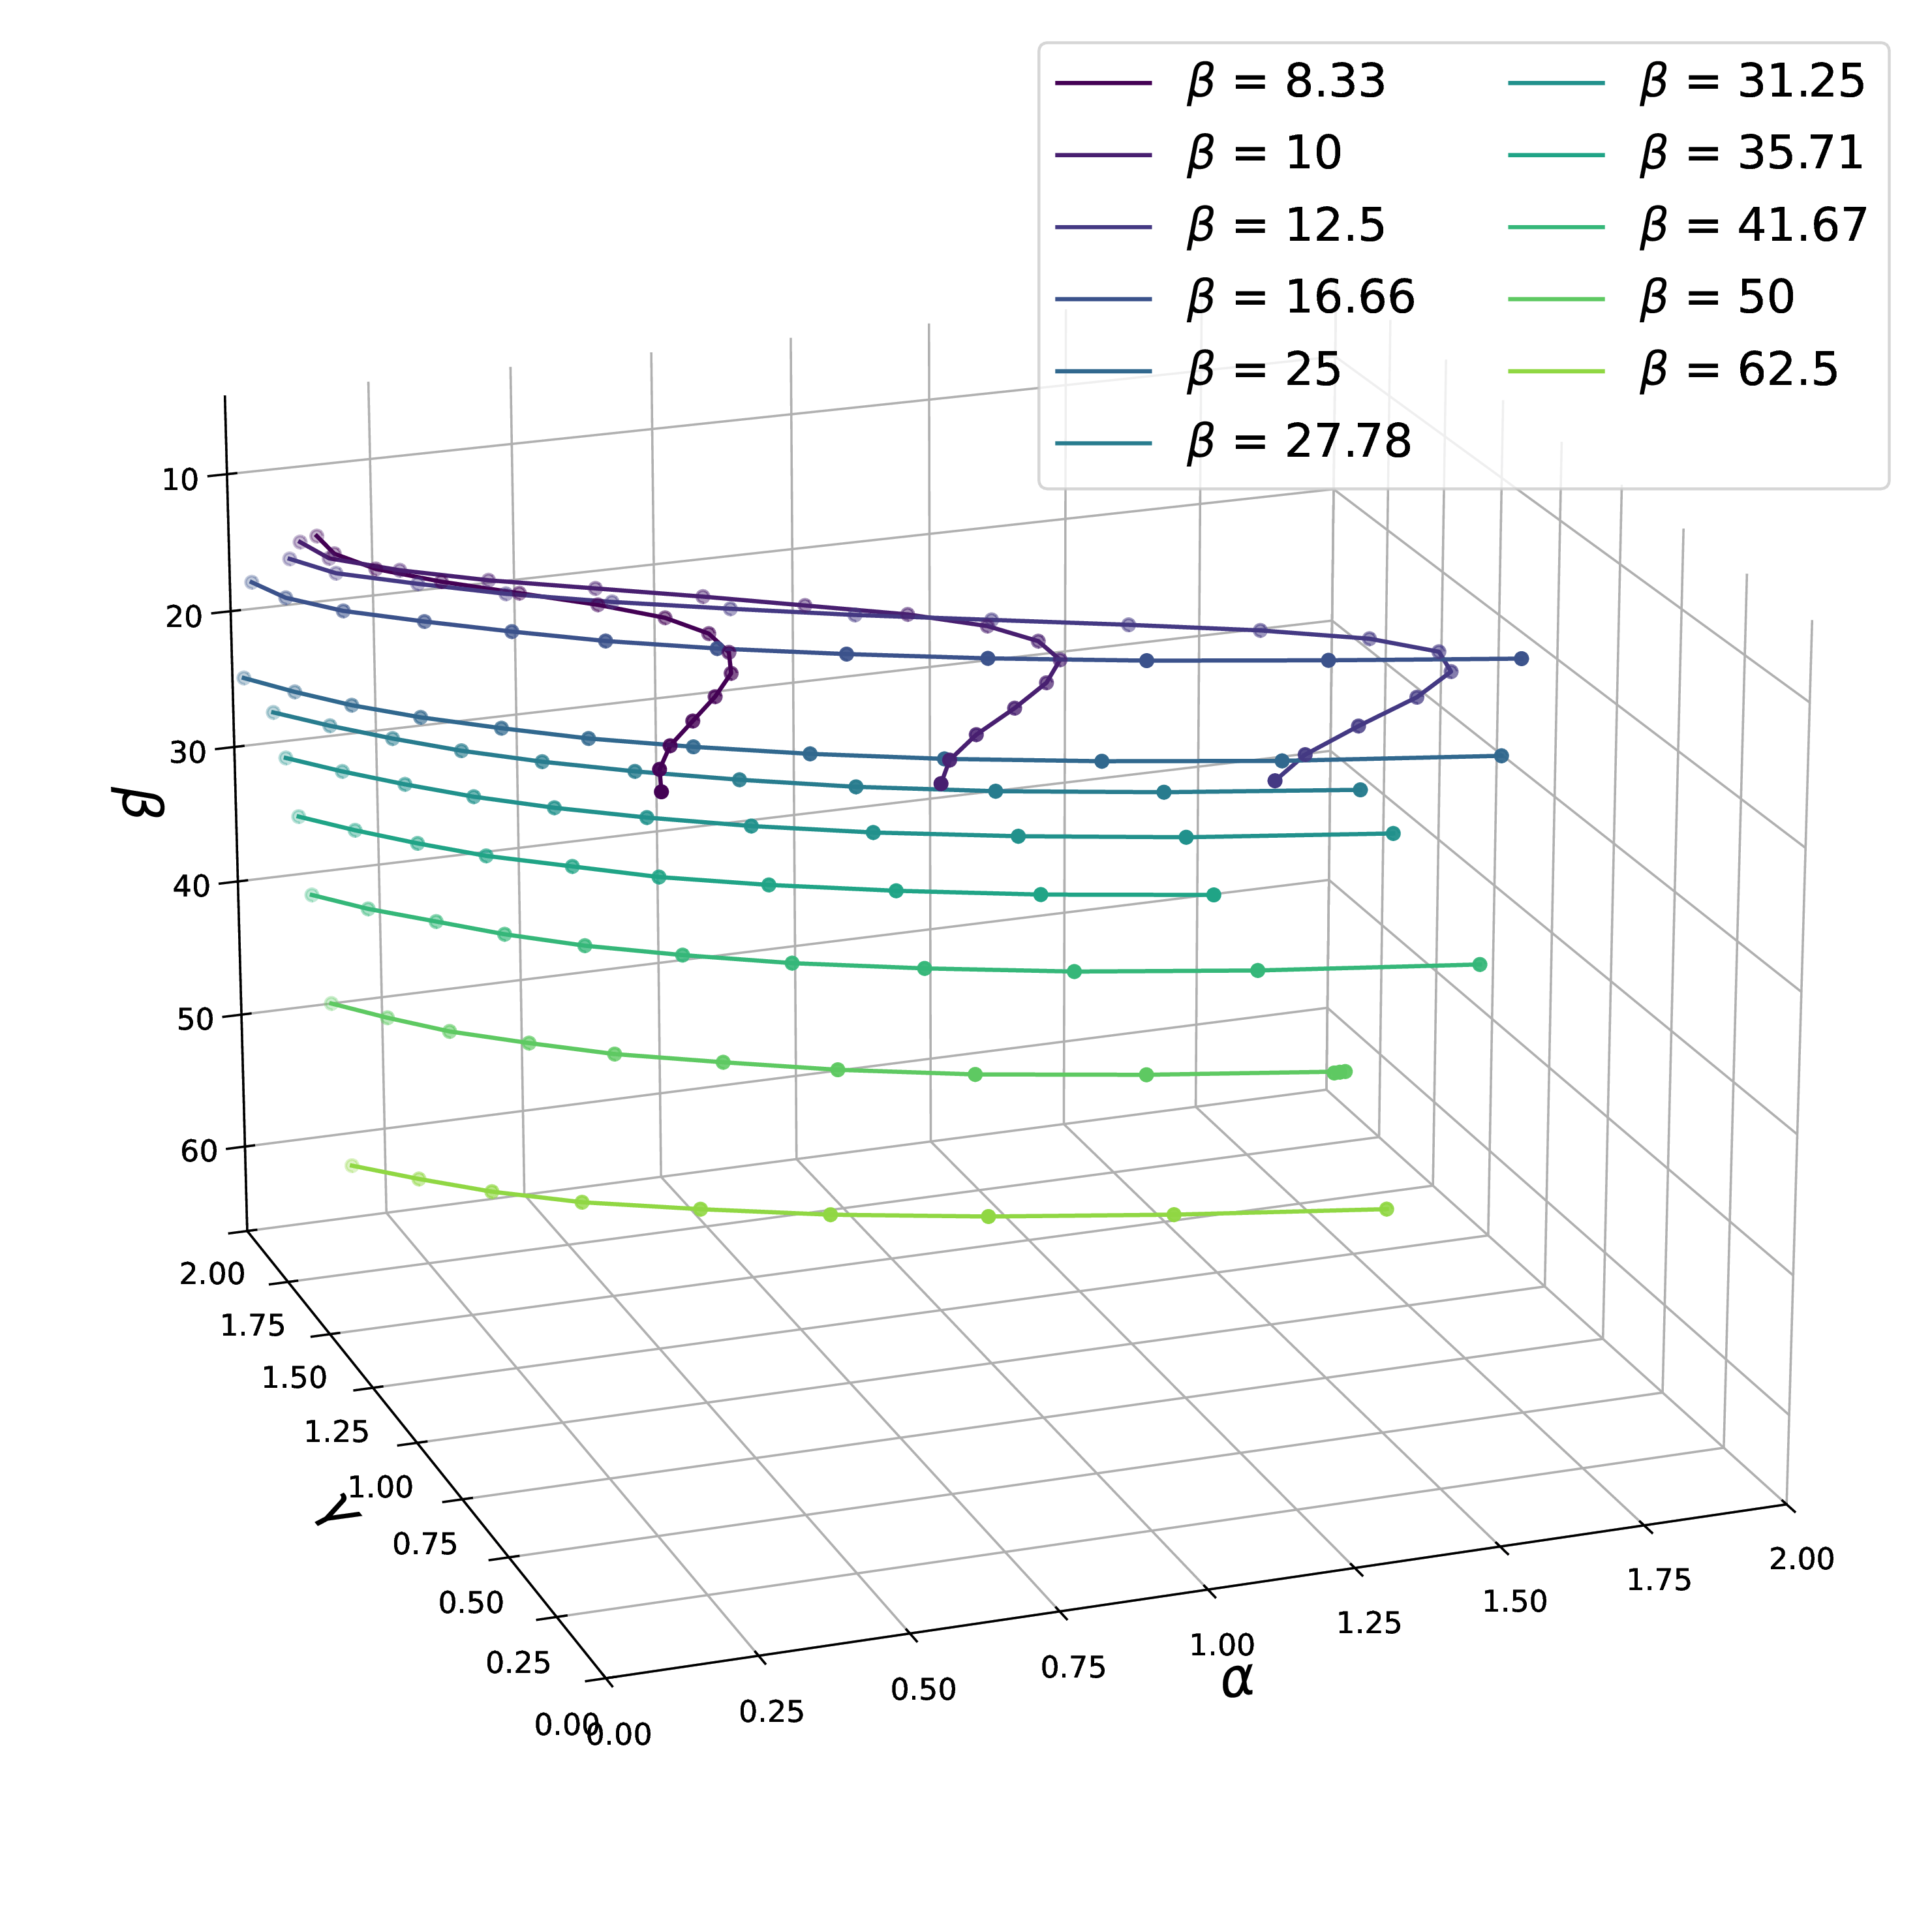
\includegraphics[width=14cm]{TexFigure/3dplot_Ns3_proj_n (0).png}}
  \caption{3-Dimension plotting of upper Figure, Fig.17,  with $\beta$ axis}
\end{figure}
\begin{figure}[htbp]
  \centerline{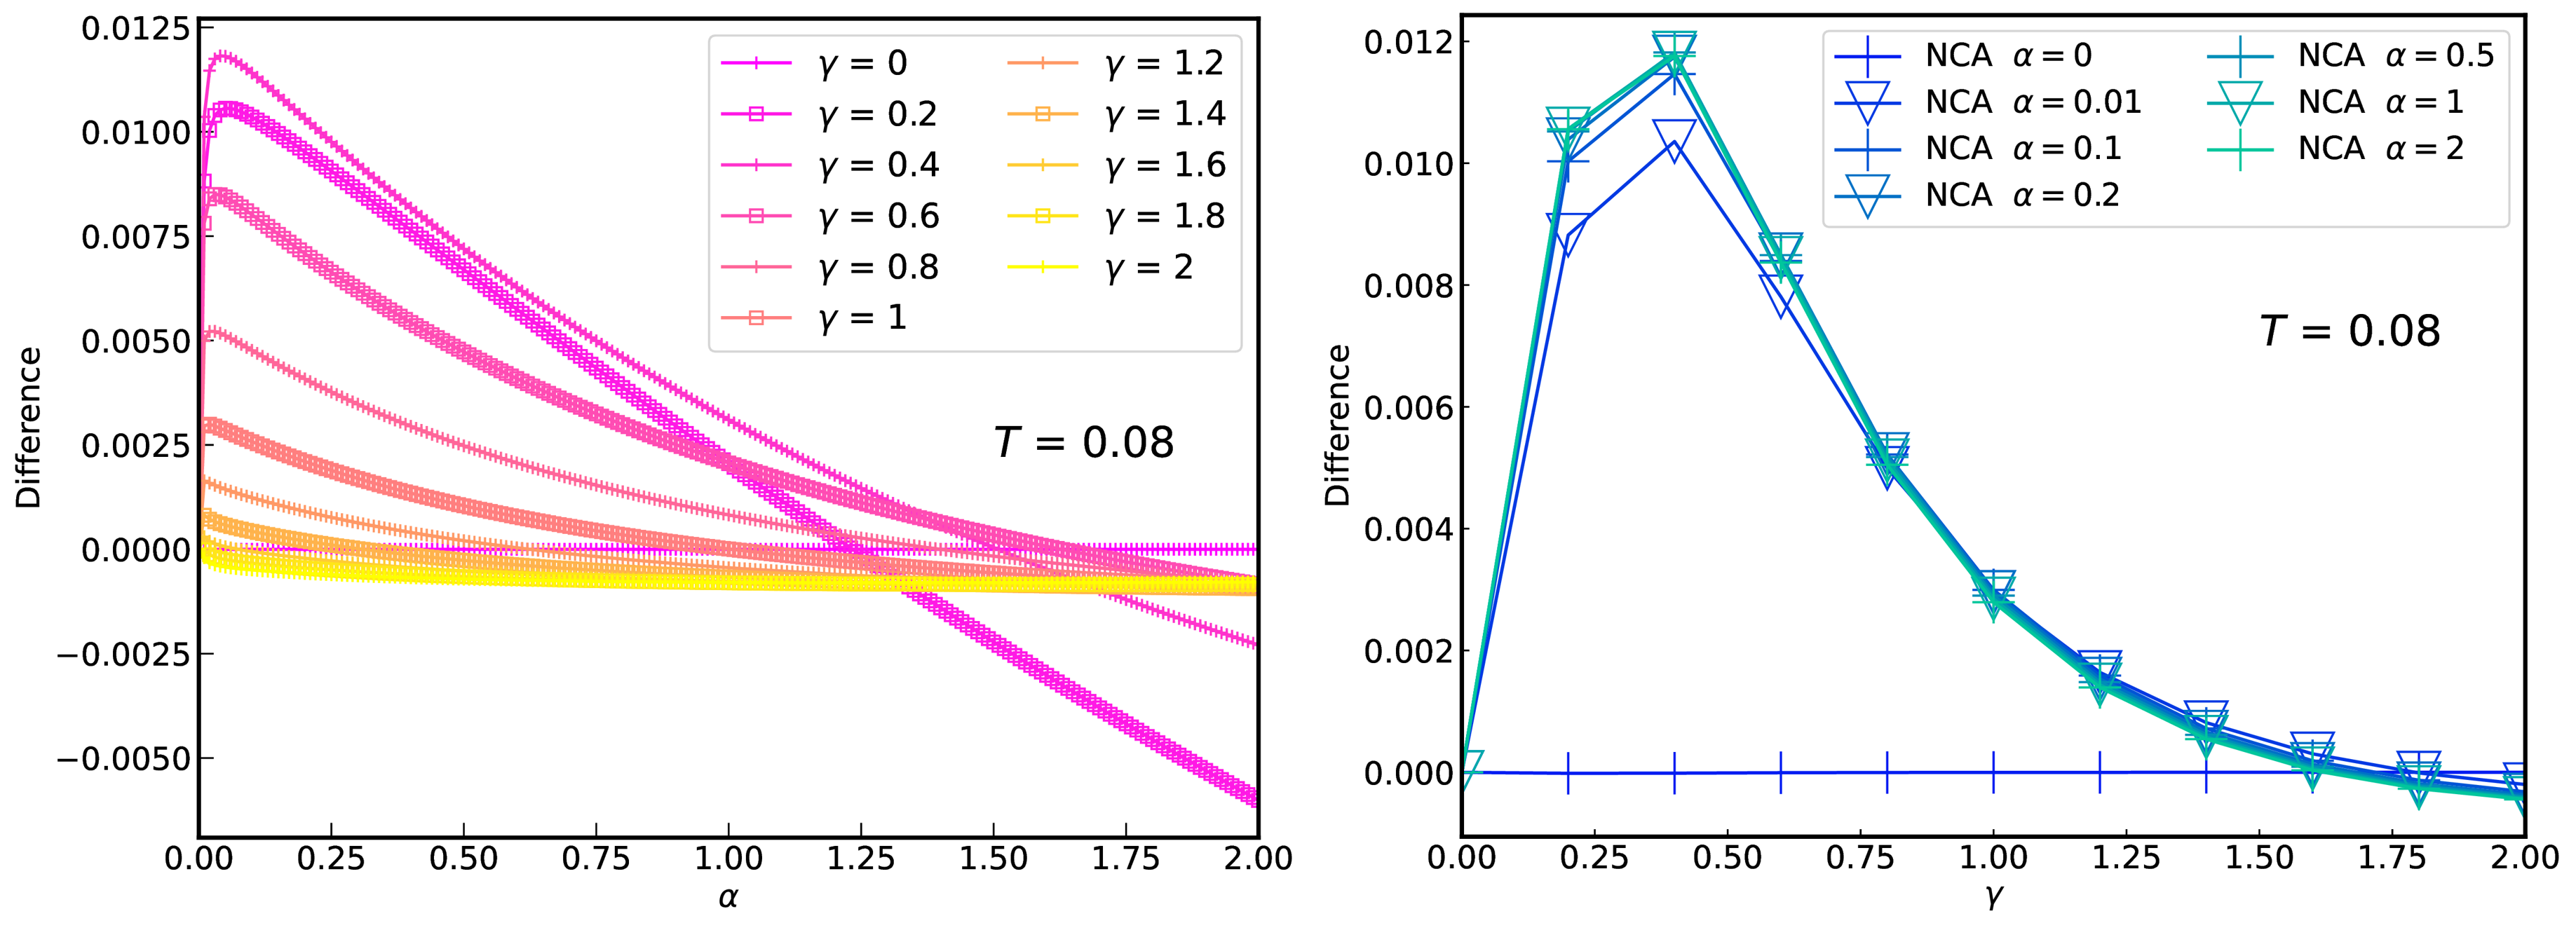
\includegraphics[width=15cm]{TexFigure/swap_fig.png}}
  \caption{The crossing picture in $\alpha$ swapping, $\gamma$ swapping}
\end{figure}
\pagebreak
\subsection{$\chi_{sp}$}
We utilize the method of calculating DC conductivity, which has formula :
\begin{flalign}
  \sigma_{DC} \approx \beta \chi_{sp}(\tau = \frac{\beta}{2})
\end{flalign}
Calculating the phase transition using the relationship between the correlation function and the DC conductivity, 
we observed the following results: Varying the $\gamma$ value at a fixed $\alpha$ value, 
conductivity tended to decrease as the interaction with the external environment increased. 
In particular, at low temperatures, the conductivity increased up to a certain value
while the rate of change decreased with respect to the $\alpha $ value.
When we fixed the $\gamma$ value and varied the $\alpha$ value, the conductivity always increased at high temperatures. 
However, at low temperatures, we observed that the conductivity decreased as the $\alpha$ value increased.
\begin{figure}[H]
  \centerline{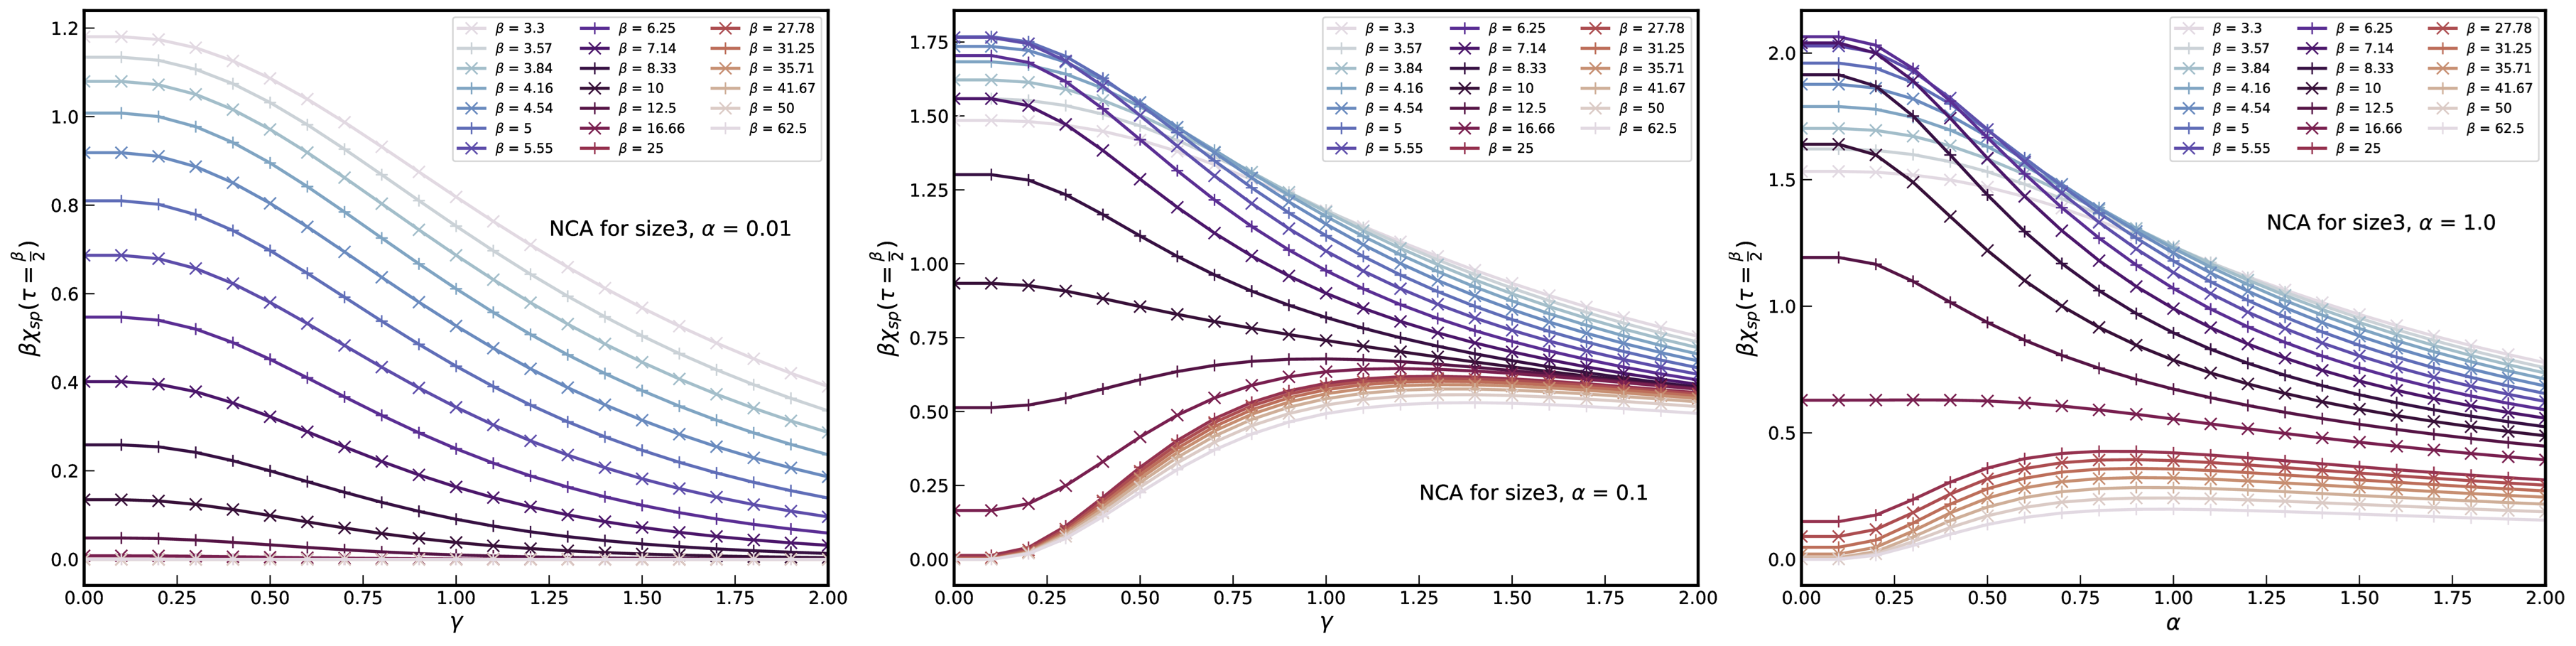
\includegraphics[width=16cm]{TexFigure/chi_gam_swp.png}}
  \centerline{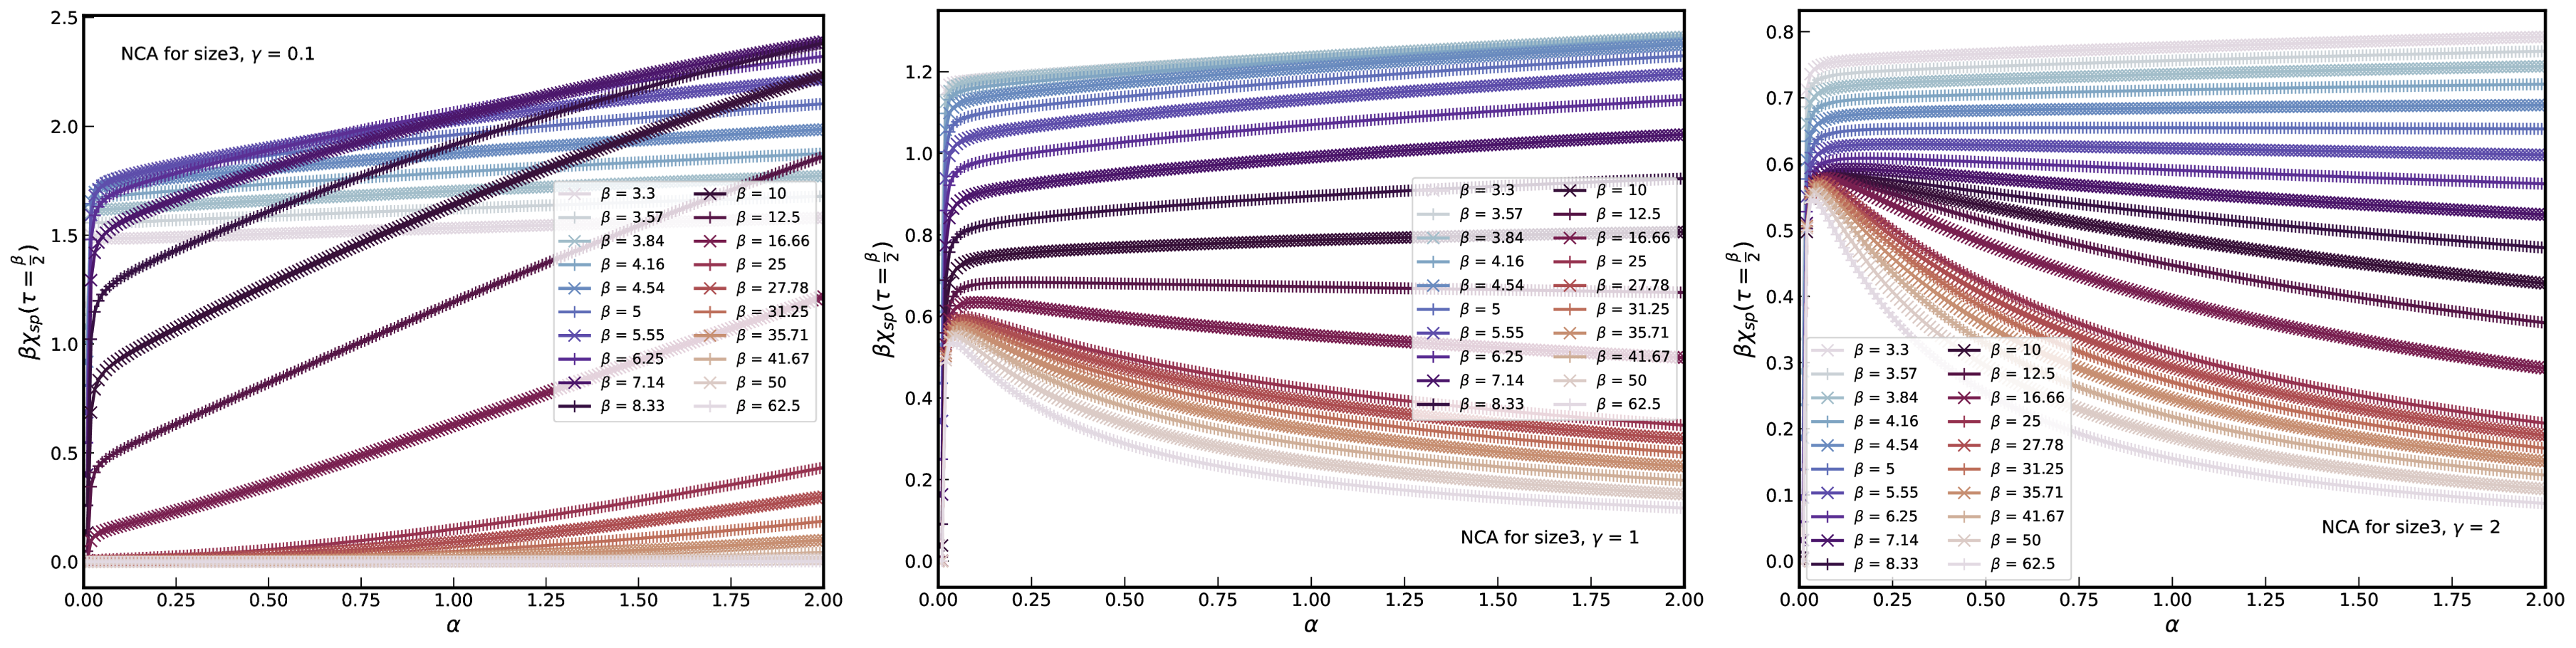
\includegraphics[width=16cm]{TexFigure/chi_alp_swp.png}}
  \caption{The crossing picture in $\chi_{sp}$ with $\gamma$ swapping and $\alpha$ swapping}
\end{figure}
\pagebreak
To observe how the conductivity changes for all $\gamma$ and $\alpha$ value conditions at a fixed temperature, 
we visualized the results using a 2D color map. At high temperatures, 
we observed that the conductivity increased as the $\gamma$ and $\alpha$ values increased. 
At low temperatures, the conductivity generally decreased as the influence of the external environment increased. 
Yet the junction energy increased, conductivity tended to increase in stronger influence from the external environment.
\begin{figure}[H]
  \centerline{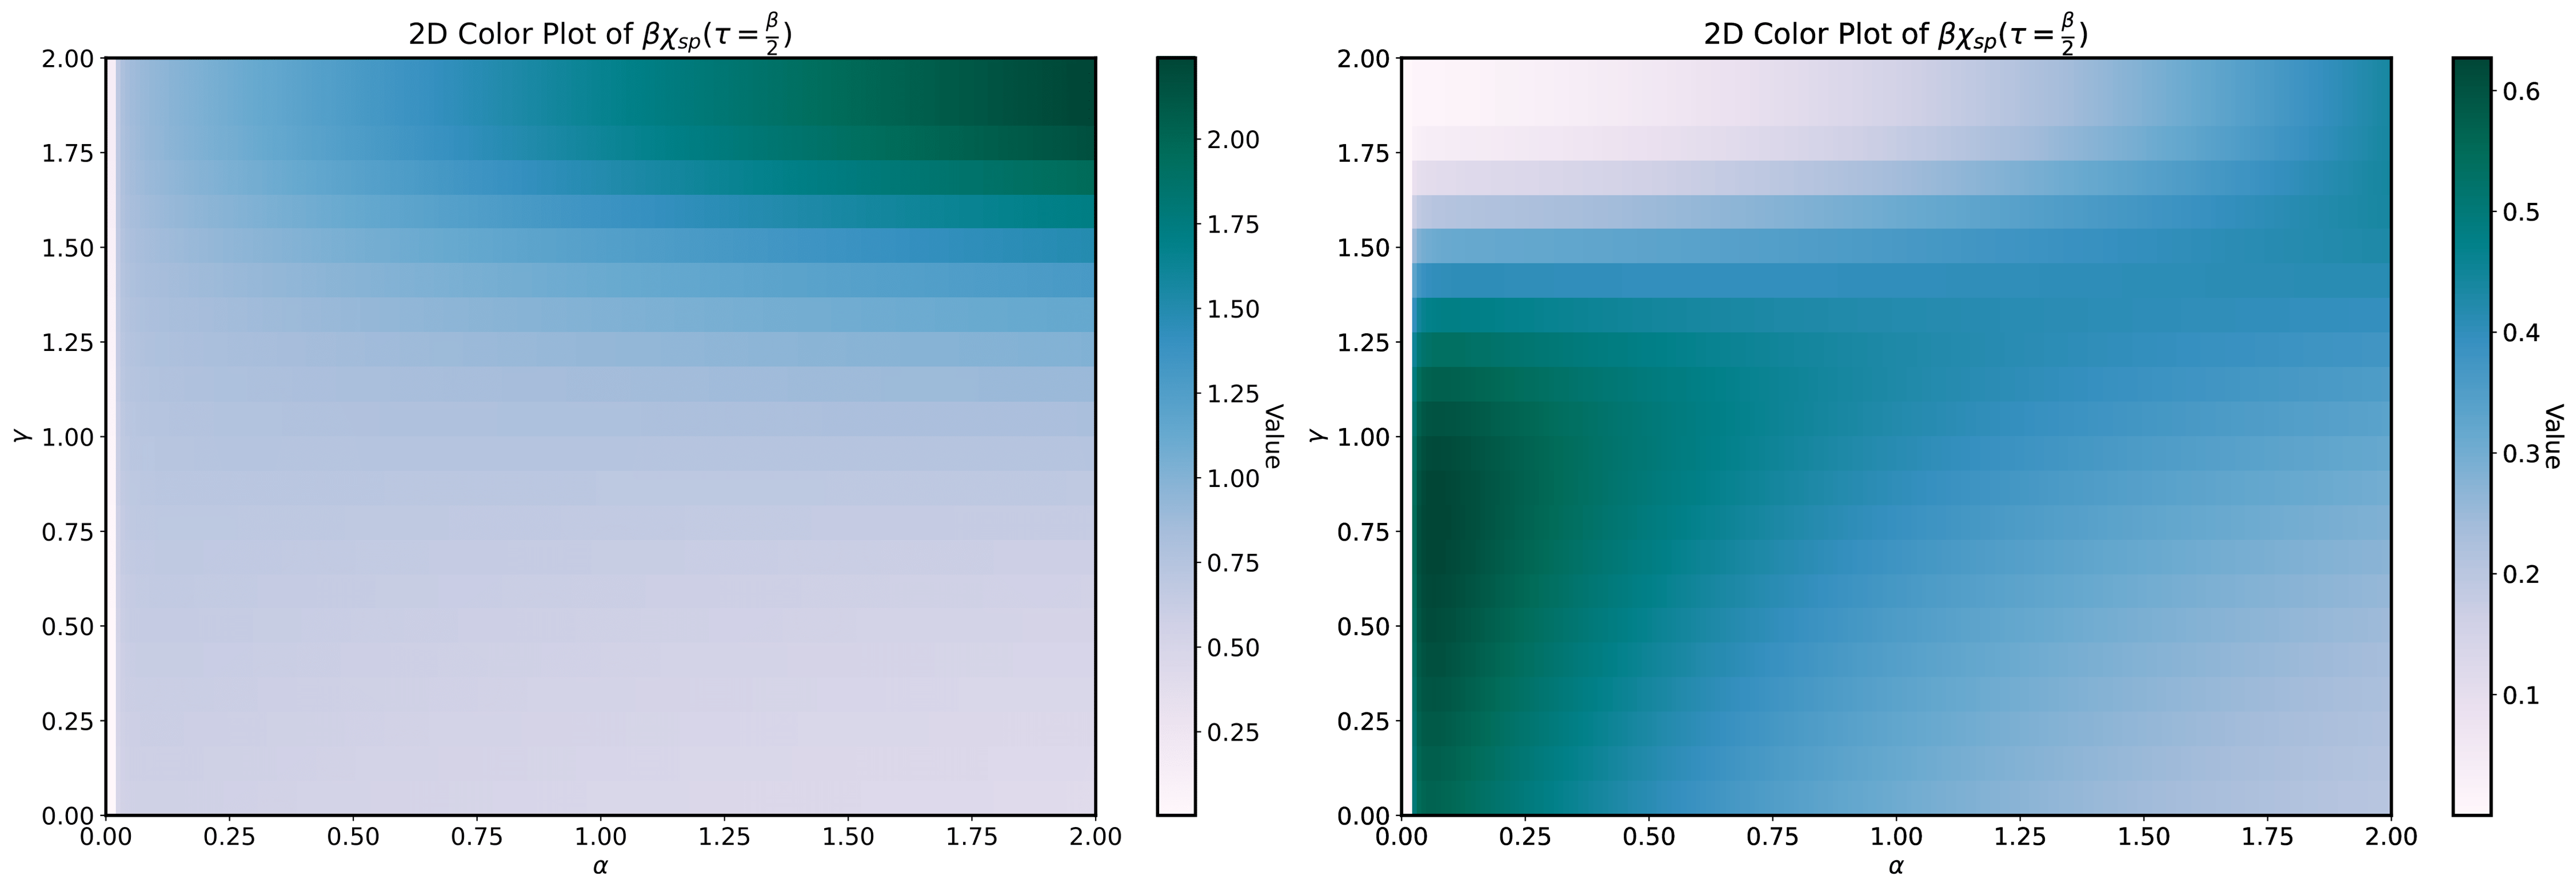
\includegraphics[width=16cm]{TexFigure/chi_color.png}}
  \caption{Colored plot for DC conductivity approximation. The simulation was performed in NCA. Left figure is in the case of $\beta=10$, Right is for $\beta=25$.
  The Josephson junction goes high conductivy as color goes deeper.}
\end{figure}
\pagebreak
\subsubsection*{$\chi_{sp}$ result from exceeded simulation range}
In the metal-insulator transition calculation using DC conductivity, 
while plotting the temperature-dependent behavior of conductivity calculated with the approximation formula varying the influencing variables, 
the point where the lines crossing corresponding to two consecutive temperatures intersect can be predicted as the phase transition point.
Within the previous set simulation range, 
the temperature-dependent conductivity approximation behavior was not clearly observed. 
Therefore, as a first attempt, we tried calculations with a wider range of $\alpha$ values while maintaining the range of $\gamma$ values. 
However, it should be noted that the size of the τ grid was reduced for faster calculation verification. 
The range conditions used are shown in the table below.
\begin{table}[htbp]
  \centering
  \renewcommand{\arraystretch}{1.2}  % 행 간격 조정
  \begin{tabular}{@{}cccc@{}}
  \toprule
  \textbf{Variables} & \textbf{Min} & \textbf{Max}  & \textbf{Interval}\\ 
  \midrule
  $\gamma$ & 0 & 2 & 0.01 \\
  $\alpha$ & 0 & 20 & 1 \\
  $\beta$ & 3.3 & 25 &  \\
  Temperature & 0.3 & 0.04 & 0.02 \\
  \bottomrule
  \end{tabular}
  \caption{Exceeded condition used for $\chi_{sp}$ calculation.}
  \end{table}
\begin{table}[htbp]
  \centering
  \renewcommand{\arraystretch}{1.2}  % 행 간격 조정
  \begin{tabular}{@{}ccc@{}}
  \toprule
  \textbf{Number} & \textbf{Interval} & \textbf{Gridsize}\\ 
  \midrule
  $\tau$ grid & [0,$\beta$] & 700 \\
  k grid & [0,K = 30000] & 30000 \\
  \bottomrule
  \end{tabular}
  \caption{Exceeded grid condition used for $\chi_{sp}$ calculation}
  \end{table}
When the calculation was performed by increasing the $\gamma$ value for a fixed $\alpha$ value, crossing points occurred according to temperature, 
and it was confirmed that the points obtained within the temperature interval converged to a specific line as the $\alpha$ value increased. 
Purple lines represent the results of OCA, and green lines represent the results of NCA. 
Based on the result, we draw the expected locations of the critical points from the results calculated by the approximation method. 
The change of $\gamma$ as a function of $\alpha$ was re-plotted using the conductivity intersection points above. 
The color of the line corresponds to each different β value.
Throughout the result, we confirmed that the reason why the prediction of the phase transition point through conductivity approximation was not possible 
in the previous calculation range was that no intersection value appeared at $\alpha$ values less than 2 at low temperatures. 
Also, we confirmed that the phase transition interval using DC conductivity decreased as the temperature decreased.
\pagebreak
\begin{figure}[H]
  \centerline{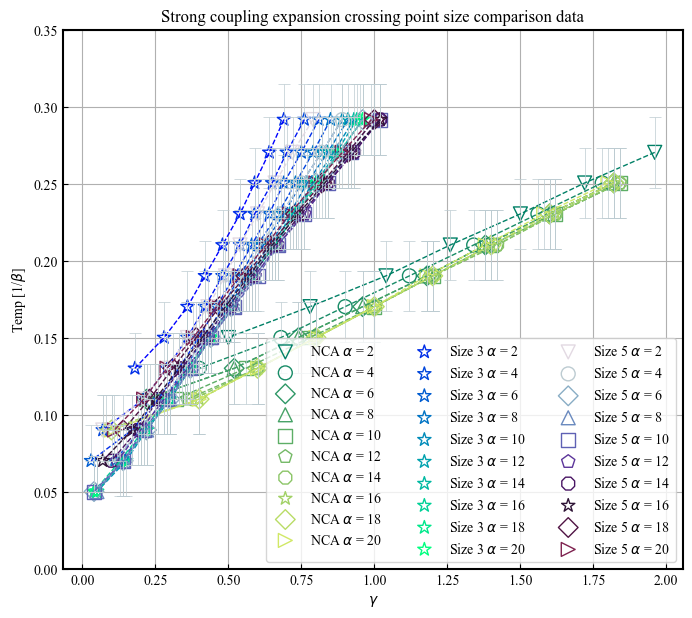
\includegraphics[width=12cm]{TexFigure/output.png}}
  \caption{Crossing points in the exceeded range. Each color represents the difference in the approximation method, 
  with green representing NCA with a matrix size of 3,  and purple representing OCA for matrix sizes 3 and 5 respectively. 
  It can be observed that the position of the line changes significantly for a matrix size of 3, i.e., a two-level energy system, 
  in the region with large $\alpha$ values.}
\end{figure}
\begin{figure}[htbp]
  \centerline{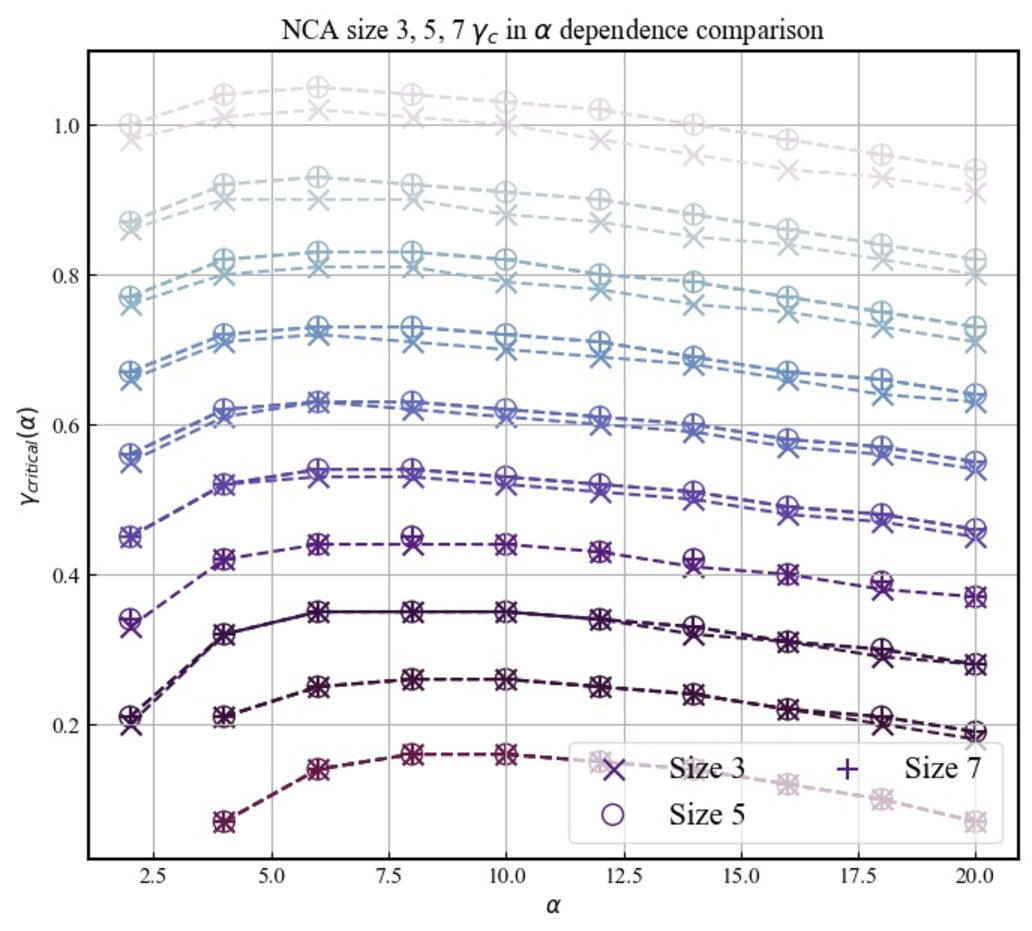
\includegraphics[width=12cm]{TexFigure/NCA_crit-7.pdf}}
  \centerline{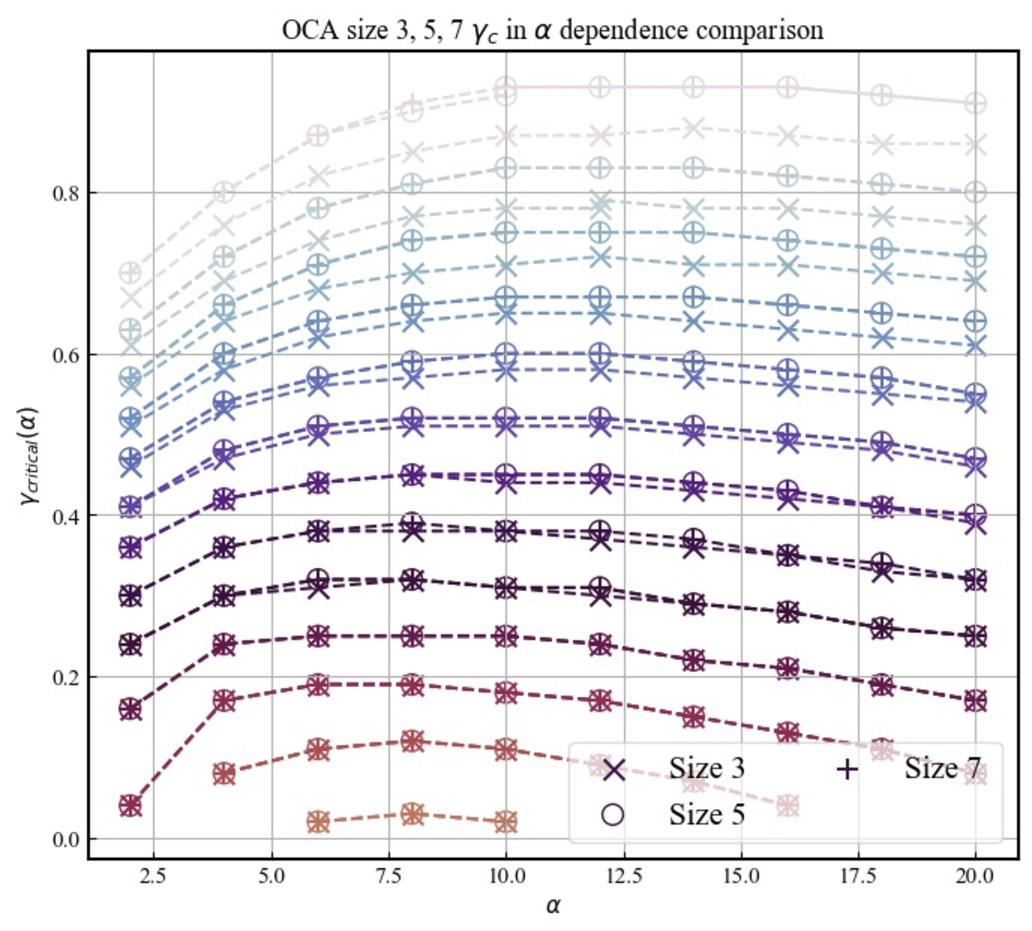
\includegraphics[width=12cm]{TexFigure/OCA_crit-7.pdf}}
  \caption{Estimated line of the criticality of the system in gamma as the function of alpha. 
  Each colored line corresponds to each temperature when the temperature range from 0.3 to 0.04 is divided into 0.02 intervals 
  from top to bottom. In the case of NCA, no critical point was observed at temperatures below 0.08.}
\end{figure}
\pagebreak
\newpage
\end{spacing}
\end{document}